\documentclass[aspectratio=169]{beamer}

\usetheme{Boadilla}
\usefonttheme{professionalfonts}
\setbeamertemplate{navigation symbols}{}
\setbeamertemplate{itemize items}[circle]
\setbeamertemplate{enumerate items}[default]
\setbeamertemplate{headline}{}

\usepackage[utf8]{inputenc}
\usepackage[T1]{fontenc}
\usepackage{lmodern}
\usepackage{amsmath}
\usepackage{booktabs}
\usepackage{tabularx}
\usepackage{array}
\usepackage{hyperref}
\usepackage[strings]{underscore}
\usepackage{listings}
\usepackage{tikz}
\usetikzlibrary{arrows.meta,positioning,fit,calc,shapes.geometric}
\usepackage{xcolor}

\definecolor{courseblue}{HTML}{12355B}
\definecolor{coursegold}{HTML}{C98A2E}
\definecolor{courseice}{HTML}{EEF3F8}
\definecolor{coursegreen}{HTML}{2F6B4F}
\definecolor{coursegray}{HTML}{4B5563}
\definecolor{codebg}{HTML}{F7F9FC}
\definecolor{codecomment}{HTML}{5E6C84}
\definecolor{codestring}{HTML}{0B6E4F}

\setbeamercolor{palette primary}{bg=courseblue,fg=white}
\setbeamercolor{palette secondary}{bg=coursegold,fg=white}
\setbeamercolor{palette tertiary}{bg=courseblue,fg=white}
\setbeamercolor{palette quaternary}{bg=coursegold,fg=white}
\setbeamercolor{structure}{fg=courseblue}
\setbeamercolor{frametitle}{bg=courseice,fg=courseblue}
\setbeamercolor{title}{fg=courseblue}
\setbeamercolor{block title}{bg=courseblue,fg=white}
\setbeamercolor{block body}{bg=courseice,fg=black}
\setbeamercolor{normal text}{fg=black,bg=white}
\setbeamercolor{alerted text}{fg=coursegold}

\setbeamerfont{footline}{size=\scriptsize}

\setbeamertemplate{footline}{
  \leavevmode
  \hbox{
    \begin{beamercolorbox}[wd=.33\paperwidth,ht=2.8ex,dp=1.2ex,leftskip=0.8em]{palette primary}%
      University of Trieste
    \end{beamercolorbox}%
    \begin{beamercolorbox}[wd=.49\paperwidth,ht=2.8ex,dp=1.2ex,center]{palette tertiary}%
      \coursename{} \textbar{} \coursecode
    \end{beamercolorbox}%
    \begin{beamercolorbox}[wd=.18\paperwidth,ht=2.8ex,dp=1.2ex,rightskip=0.8em plus1fil]{palette secondary}%
      \insertframenumber{} / \inserttotalframenumber
    \end{beamercolorbox}%
  }
}

\hypersetup{
  colorlinks=true,
  linkcolor=courseblue,
  urlcolor=coursegreen
}

\lstdefinestyle{coursepython}{
  language=Python,
  basicstyle=\ttfamily\footnotesize,
  keywordstyle=\color{courseblue}\bfseries,
  commentstyle=\color{codecomment}\itshape,
  stringstyle=\color{codestring},
  showstringspaces=false,
  columns=fullflexible,
  keepspaces=true,
  frame=single,
  framerule=0.6pt,
  rulecolor=\color{courseblue},
  backgroundcolor=\color{codebg},
  xleftmargin=0.4em,
  xrightmargin=0.4em,
  aboveskip=0.4em,
  belowskip=0.2em
}

\newcommand{\coursename}{Data-driven Systems Engineering}
\newcommand{\coursecode}{440MI / 305SM}
\newcommand{\coursefooter}{}

\newcommand{\learninggoals}[1]{
  \begin{block}{Learning goals}
  #1
  \end{block}
}

\newcommand{\repoactivity}[1]{
  \begin{block}{Repo activity}
  #1
  \end{block}
}

\newcommand{\readinglist}[1]{
  \begin{block}{Papers and materials}
  {\footnotesize #1}
  \end{block}
}

\newcommand{\coursecontextframe}[5]{
  \begin{frame}{Course Map and Running Cases}
  \centering
  \begin{tikzpicture}[node distance=0.28cm]
  \node[flowbox, minimum width=1.45cm, minimum height=0.8cm] (problem) {\scriptsize Problem};
  \node[flowbox, minimum width=1.45cm, minimum height=0.8cm, right=of problem] (data) {\scriptsize Data};
  \node[flowbox, minimum width=1.45cm, minimum height=0.8cm, right=of data] (features) {\scriptsize Features};
  \node[flowbox, minimum width=1.45cm, minimum height=0.8cm, right=of features] (model) {\scriptsize Model};
  \node[flowbox, minimum width=1.45cm, minimum height=0.8cm, right=of model] (interface) {\scriptsize Interface};
  \node[flowbox, minimum width=1.45cm, minimum height=0.8cm, right=of interface] (delivery) {\scriptsize Delivery};
  \node[flowbox, minimum width=1.45cm, minimum height=0.8cm, right=of delivery] (monitor) {\scriptsize Monitor};
  \node[accentbox, minimum width=1.6cm, minimum height=0.8cm, right=of monitor] (evolution) {\scriptsize Evolution};
  \foreach \a/\b in {problem/data,data/features,features/model,model/interface,interface/delivery,delivery/monitor,monitor/evolution} {
    \draw[arrow] (\a) -- (\b);
  }
  \end{tikzpicture}

  \vspace{0.5em}
  \begin{block}{Today in the course}
  \textbf{Focus:} #1

  \textbf{Bridge:} #2
  \end{block}

  \begin{columns}[T]
  \column{0.48\textwidth}
  \begin{block}{Fraud case}
  {\footnotesize #3}
  \end{block}
  \column{0.48\textwidth}
  \begin{block}{Pasteurization case}
  {\footnotesize #4}
  \end{block}
  \end{columns}

  \vspace{0.3em}
  {\footnotesize \textbf{Course thread:} #5}
  \coursefooter
  \end{frame}
}

\newcommand{\classclosingframe}[4]{
  \begin{frame}{From This Class to the Next}
  \begin{block}{What stays with us}
  #1
  \end{block}

  \begin{columns}[T]
  \column{0.48\textwidth}
  \begin{block}{Project use}
  {\footnotesize #2}
  \end{block}
  \column{0.48\textwidth}
  \begin{block}{Next connection}
  {\footnotesize #3}
  \end{block}
  \end{columns}

  \vspace{0.3em}
  {\footnotesize \textbf{Course thread:} #4}
  \coursefooter
  \end{frame}
}

\tikzset{
  flowbox/.style={
    rounded corners=3pt,
    draw=courseblue,
    fill=courseice,
    very thick,
    minimum width=2.2cm,
    minimum height=0.9cm,
    align=center,
    font=\small
  },
  accentbox/.style={
    rounded corners=3pt,
    draw=coursegold,
    fill=coursegold!15,
    very thick,
    minimum width=2.2cm,
    minimum height=0.9cm,
    align=center,
    font=\small
  },
  arrow/.style={
    -{Latex[length=2.5mm,width=2mm]},
    thick,
    draw=courseblue
  }
}

% Visual layer on top of common.tex: tiles, icons, a progress-strip section divider, and a footer
% strip that defines the concepts appearing for the first time on each slide.
% Same look as the Class 20 deck. Load with:  \documentclass[aspectratio=169]{beamer}

\usetheme{Boadilla}
\usefonttheme{professionalfonts}
\setbeamertemplate{navigation symbols}{}
\setbeamertemplate{itemize items}[circle]
\setbeamertemplate{enumerate items}[default]
\setbeamertemplate{headline}{}

\usepackage[utf8]{inputenc}
\usepackage[T1]{fontenc}
\usepackage{lmodern}
\usepackage{amsmath}
\usepackage{booktabs}
\usepackage{tabularx}
\usepackage{array}
\usepackage{hyperref}
\usepackage[strings]{underscore}
\usepackage{listings}
\usepackage{tikz}
\usetikzlibrary{arrows.meta,positioning,fit,calc,shapes.geometric}
\usepackage{xcolor}

\definecolor{courseblue}{HTML}{12355B}
\definecolor{coursegold}{HTML}{C98A2E}
\definecolor{courseice}{HTML}{EEF3F8}
\definecolor{coursegreen}{HTML}{2F6B4F}
\definecolor{coursegray}{HTML}{4B5563}
\definecolor{codebg}{HTML}{F7F9FC}
\definecolor{codecomment}{HTML}{5E6C84}
\definecolor{codestring}{HTML}{0B6E4F}

\setbeamercolor{palette primary}{bg=courseblue,fg=white}
\setbeamercolor{palette secondary}{bg=coursegold,fg=white}
\setbeamercolor{palette tertiary}{bg=courseblue,fg=white}
\setbeamercolor{palette quaternary}{bg=coursegold,fg=white}
\setbeamercolor{structure}{fg=courseblue}
\setbeamercolor{frametitle}{bg=courseice,fg=courseblue}
\setbeamercolor{title}{fg=courseblue}
\setbeamercolor{block title}{bg=courseblue,fg=white}
\setbeamercolor{block body}{bg=courseice,fg=black}
\setbeamercolor{normal text}{fg=black,bg=white}
\setbeamercolor{alerted text}{fg=coursegold}

\setbeamerfont{footline}{size=\scriptsize}

\setbeamertemplate{footline}{
  \leavevmode
  \hbox{
    \begin{beamercolorbox}[wd=.33\paperwidth,ht=2.8ex,dp=1.2ex,leftskip=0.8em]{palette primary}%
      University of Trieste
    \end{beamercolorbox}%
    \begin{beamercolorbox}[wd=.49\paperwidth,ht=2.8ex,dp=1.2ex,center]{palette tertiary}%
      \coursename{} \textbar{} \coursecode
    \end{beamercolorbox}%
    \begin{beamercolorbox}[wd=.18\paperwidth,ht=2.8ex,dp=1.2ex,rightskip=0.8em plus1fil]{palette secondary}%
      \insertframenumber{} / \inserttotalframenumber
    \end{beamercolorbox}%
  }
}

\hypersetup{
  colorlinks=true,
  linkcolor=courseblue,
  urlcolor=coursegreen
}

\lstdefinestyle{coursepython}{
  language=Python,
  basicstyle=\ttfamily\footnotesize,
  keywordstyle=\color{courseblue}\bfseries,
  commentstyle=\color{codecomment}\itshape,
  stringstyle=\color{codestring},
  showstringspaces=false,
  columns=fullflexible,
  keepspaces=true,
  frame=single,
  framerule=0.6pt,
  rulecolor=\color{courseblue},
  backgroundcolor=\color{codebg},
  xleftmargin=0.4em,
  xrightmargin=0.4em,
  aboveskip=0.4em,
  belowskip=0.2em
}

\newcommand{\coursename}{Data-driven Systems Engineering}
\newcommand{\coursecode}{440MI / 305SM}
\newcommand{\coursefooter}{}

\newcommand{\learninggoals}[1]{
  \begin{block}{Learning goals}
  #1
  \end{block}
}

\newcommand{\repoactivity}[1]{
  \begin{block}{Repo activity}
  #1
  \end{block}
}

\newcommand{\readinglist}[1]{
  \begin{block}{Papers and materials}
  {\footnotesize #1}
  \end{block}
}

\newcommand{\coursecontextframe}[5]{
  \begin{frame}{Course Map and Running Cases}
  \centering
  \begin{tikzpicture}[node distance=0.28cm]
  \node[flowbox, minimum width=1.45cm, minimum height=0.8cm] (problem) {\scriptsize Problem};
  \node[flowbox, minimum width=1.45cm, minimum height=0.8cm, right=of problem] (data) {\scriptsize Data};
  \node[flowbox, minimum width=1.45cm, minimum height=0.8cm, right=of data] (features) {\scriptsize Features};
  \node[flowbox, minimum width=1.45cm, minimum height=0.8cm, right=of features] (model) {\scriptsize Model};
  \node[flowbox, minimum width=1.45cm, minimum height=0.8cm, right=of model] (interface) {\scriptsize Interface};
  \node[flowbox, minimum width=1.45cm, minimum height=0.8cm, right=of interface] (delivery) {\scriptsize Delivery};
  \node[flowbox, minimum width=1.45cm, minimum height=0.8cm, right=of delivery] (monitor) {\scriptsize Monitor};
  \node[accentbox, minimum width=1.6cm, minimum height=0.8cm, right=of monitor] (evolution) {\scriptsize Evolution};
  \foreach \a/\b in {problem/data,data/features,features/model,model/interface,interface/delivery,delivery/monitor,monitor/evolution} {
    \draw[arrow] (\a) -- (\b);
  }
  \end{tikzpicture}

  \vspace{0.5em}
  \begin{block}{Today in the course}
  \textbf{Focus:} #1

  \textbf{Bridge:} #2
  \end{block}

  \begin{columns}[T]
  \column{0.48\textwidth}
  \begin{block}{Fraud case}
  {\footnotesize #3}
  \end{block}
  \column{0.48\textwidth}
  \begin{block}{Pasteurization case}
  {\footnotesize #4}
  \end{block}
  \end{columns}

  \vspace{0.3em}
  {\footnotesize \textbf{Course thread:} #5}
  \coursefooter
  \end{frame}
}

\newcommand{\classclosingframe}[4]{
  \begin{frame}{From This Class to the Next}
  \begin{block}{What stays with us}
  #1
  \end{block}

  \begin{columns}[T]
  \column{0.48\textwidth}
  \begin{block}{Project use}
  {\footnotesize #2}
  \end{block}
  \column{0.48\textwidth}
  \begin{block}{Next connection}
  {\footnotesize #3}
  \end{block}
  \end{columns}

  \vspace{0.3em}
  {\footnotesize \textbf{Course thread:} #4}
  \coursefooter
  \end{frame}
}

\tikzset{
  flowbox/.style={
    rounded corners=3pt,
    draw=courseblue,
    fill=courseice,
    very thick,
    minimum width=2.2cm,
    minimum height=0.9cm,
    align=center,
    font=\small
  },
  accentbox/.style={
    rounded corners=3pt,
    draw=coursegold,
    fill=coursegold!15,
    very thick,
    minimum width=2.2cm,
    minimum height=0.9cm,
    align=center,
    font=\small
  },
  arrow/.style={
    -{Latex[length=2.5mm,width=2mm]},
    thick,
    draw=courseblue
  }
}
  % Visual layer on top of common.tex: tiles, icons, a progress-strip section divider, and a footer
% strip that defines the concepts appearing for the first time on each slide.
% Same look as the Class 20 deck. Load with:  \documentclass[aspectratio=169]{beamer}

\usetheme{Boadilla}
\usefonttheme{professionalfonts}
\setbeamertemplate{navigation symbols}{}
\setbeamertemplate{itemize items}[circle]
\setbeamertemplate{enumerate items}[default]
\setbeamertemplate{headline}{}

\usepackage[utf8]{inputenc}
\usepackage[T1]{fontenc}
\usepackage{lmodern}
\usepackage{amsmath}
\usepackage{booktabs}
\usepackage{tabularx}
\usepackage{array}
\usepackage{hyperref}
\usepackage[strings]{underscore}
\usepackage{listings}
\usepackage{tikz}
\usetikzlibrary{arrows.meta,positioning,fit,calc,shapes.geometric}
\usepackage{xcolor}

\definecolor{courseblue}{HTML}{12355B}
\definecolor{coursegold}{HTML}{C98A2E}
\definecolor{courseice}{HTML}{EEF3F8}
\definecolor{coursegreen}{HTML}{2F6B4F}
\definecolor{coursegray}{HTML}{4B5563}
\definecolor{codebg}{HTML}{F7F9FC}
\definecolor{codecomment}{HTML}{5E6C84}
\definecolor{codestring}{HTML}{0B6E4F}

\setbeamercolor{palette primary}{bg=courseblue,fg=white}
\setbeamercolor{palette secondary}{bg=coursegold,fg=white}
\setbeamercolor{palette tertiary}{bg=courseblue,fg=white}
\setbeamercolor{palette quaternary}{bg=coursegold,fg=white}
\setbeamercolor{structure}{fg=courseblue}
\setbeamercolor{frametitle}{bg=courseice,fg=courseblue}
\setbeamercolor{title}{fg=courseblue}
\setbeamercolor{block title}{bg=courseblue,fg=white}
\setbeamercolor{block body}{bg=courseice,fg=black}
\setbeamercolor{normal text}{fg=black,bg=white}
\setbeamercolor{alerted text}{fg=coursegold}

\setbeamerfont{footline}{size=\scriptsize}

\setbeamertemplate{footline}{
  \leavevmode
  \hbox{
    \begin{beamercolorbox}[wd=.33\paperwidth,ht=2.8ex,dp=1.2ex,leftskip=0.8em]{palette primary}%
      University of Trieste
    \end{beamercolorbox}%
    \begin{beamercolorbox}[wd=.49\paperwidth,ht=2.8ex,dp=1.2ex,center]{palette tertiary}%
      \coursename{} \textbar{} \coursecode
    \end{beamercolorbox}%
    \begin{beamercolorbox}[wd=.18\paperwidth,ht=2.8ex,dp=1.2ex,rightskip=0.8em plus1fil]{palette secondary}%
      \insertframenumber{} / \inserttotalframenumber
    \end{beamercolorbox}%
  }
}

\hypersetup{
  colorlinks=true,
  linkcolor=courseblue,
  urlcolor=coursegreen
}

\lstdefinestyle{coursepython}{
  language=Python,
  basicstyle=\ttfamily\footnotesize,
  keywordstyle=\color{courseblue}\bfseries,
  commentstyle=\color{codecomment}\itshape,
  stringstyle=\color{codestring},
  showstringspaces=false,
  columns=fullflexible,
  keepspaces=true,
  frame=single,
  framerule=0.6pt,
  rulecolor=\color{courseblue},
  backgroundcolor=\color{codebg},
  xleftmargin=0.4em,
  xrightmargin=0.4em,
  aboveskip=0.4em,
  belowskip=0.2em
}

\newcommand{\coursename}{Data-driven Systems Engineering}
\newcommand{\coursecode}{440MI / 305SM}
\newcommand{\coursefooter}{}

\newcommand{\learninggoals}[1]{
  \begin{block}{Learning goals}
  #1
  \end{block}
}

\newcommand{\repoactivity}[1]{
  \begin{block}{Repo activity}
  #1
  \end{block}
}

\newcommand{\readinglist}[1]{
  \begin{block}{Papers and materials}
  {\footnotesize #1}
  \end{block}
}

\newcommand{\coursecontextframe}[5]{
  \begin{frame}{Course Map and Running Cases}
  \centering
  \begin{tikzpicture}[node distance=0.28cm]
  \node[flowbox, minimum width=1.45cm, minimum height=0.8cm] (problem) {\scriptsize Problem};
  \node[flowbox, minimum width=1.45cm, minimum height=0.8cm, right=of problem] (data) {\scriptsize Data};
  \node[flowbox, minimum width=1.45cm, minimum height=0.8cm, right=of data] (features) {\scriptsize Features};
  \node[flowbox, minimum width=1.45cm, minimum height=0.8cm, right=of features] (model) {\scriptsize Model};
  \node[flowbox, minimum width=1.45cm, minimum height=0.8cm, right=of model] (interface) {\scriptsize Interface};
  \node[flowbox, minimum width=1.45cm, minimum height=0.8cm, right=of interface] (delivery) {\scriptsize Delivery};
  \node[flowbox, minimum width=1.45cm, minimum height=0.8cm, right=of delivery] (monitor) {\scriptsize Monitor};
  \node[accentbox, minimum width=1.6cm, minimum height=0.8cm, right=of monitor] (evolution) {\scriptsize Evolution};
  \foreach \a/\b in {problem/data,data/features,features/model,model/interface,interface/delivery,delivery/monitor,monitor/evolution} {
    \draw[arrow] (\a) -- (\b);
  }
  \end{tikzpicture}

  \vspace{0.5em}
  \begin{block}{Today in the course}
  \textbf{Focus:} #1

  \textbf{Bridge:} #2
  \end{block}

  \begin{columns}[T]
  \column{0.48\textwidth}
  \begin{block}{Fraud case}
  {\footnotesize #3}
  \end{block}
  \column{0.48\textwidth}
  \begin{block}{Pasteurization case}
  {\footnotesize #4}
  \end{block}
  \end{columns}

  \vspace{0.3em}
  {\footnotesize \textbf{Course thread:} #5}
  \coursefooter
  \end{frame}
}

\newcommand{\classclosingframe}[4]{
  \begin{frame}{From This Class to the Next}
  \begin{block}{What stays with us}
  #1
  \end{block}

  \begin{columns}[T]
  \column{0.48\textwidth}
  \begin{block}{Project use}
  {\footnotesize #2}
  \end{block}
  \column{0.48\textwidth}
  \begin{block}{Next connection}
  {\footnotesize #3}
  \end{block}
  \end{columns}

  \vspace{0.3em}
  {\footnotesize \textbf{Course thread:} #4}
  \coursefooter
  \end{frame}
}

\tikzset{
  flowbox/.style={
    rounded corners=3pt,
    draw=courseblue,
    fill=courseice,
    very thick,
    minimum width=2.2cm,
    minimum height=0.9cm,
    align=center,
    font=\small
  },
  accentbox/.style={
    rounded corners=3pt,
    draw=coursegold,
    fill=coursegold!15,
    very thick,
    minimum width=2.2cm,
    minimum height=0.9cm,
    align=center,
    font=\small
  },
  arrow/.style={
    -{Latex[length=2.5mm,width=2mm]},
    thick,
    draw=courseblue
  }
}
  % Visual layer on top of common.tex: tiles, icons, a progress-strip section divider, and a footer
% strip that defines the concepts appearing for the first time on each slide.
% Same look as the Class 20 deck. Load with:  \input{common}  \input{common_visual}
%
% Before the first \sectiondivider, a deck must define
%   \sectioncount   the number of sections, e.g. 4
%   \sectionlabels  a \foreach list of number/label pairs, e.g. 1/Need,2/Testable,3/Manage,4/Practice
% Icons come from the fontawesome5 package (Font Awesome 5 Free), e.g. \faIcon{robot}.

\usepackage{colortbl}
\usepackage{fontawesome5}
\usetikzlibrary{backgrounds}

% Slides read better without automatic hyphenation.
\hyphenpenalty=10000
\exhyphenpenalty=10000

\definecolor{coursered}{HTML}{A23B2A}
\newcommand{\goldink}{\color{coursegold!65!black}}

\tikzset{
  tile/.style={rounded corners=4pt, fill=courseice, draw=none, align=center, font=\footnotesize, inner sep=5pt},
  tileblue/.style={tile, fill=white, draw=courseblue!55, thick},
  tilegold/.style={tile, fill=coursegold!14, draw=coursegold, thick},
  tilegreen/.style={tile, fill=coursegreen!10, draw=coursegreen!70, thick},
  tilered/.style={tile, fill=coursered!8, draw=coursered!70, thick},
  tilegray/.style={tile, fill=white, draw=coursegray!55, thick, dashed},
  tag/.style={rounded corners=2pt, fill=coursegold, text=white, font=\bfseries\tiny, inner sep=2.5pt},
  chip/.style={rounded corners=3pt, fill=courseblue, text=white, font=\footnotesize\bfseries, align=center, inner sep=4pt},
  note/.style={font=\scriptsize, text=coursegray, align=left},
  arrowgold/.style={-{Latex[length=2.5mm,width=2mm]}, thick, draw=coursegold},
  arrowred/.style={-{Latex[length=2.5mm,width=2mm]}, thick, draw=coursered},
  arrowgreen/.style={-{Latex[length=2.5mm,width=2mm]}, thick, draw=coursegreen},
  arrowgray/.style={-{Latex[length=2mm,width=1.6mm]}, thick, draw=coursegray!70},
}

% A round icon badge, drawn inside a tikzpicture: x y colour icon
\newcommand{\badge}[4]{%
  \node[circle, fill=#3, text=white, minimum size=0.85cm, inner sep=0pt] at (#1,#2) {\large\faIcon{#4}};
}

% Inline tags for the kind of requirement.
\newcommand{\Ftag}{\colorbox{courseblue}{\color{white}\bfseries\scriptsize\ \ F\ \ }}
\newcommand{\NFtag}{\colorbox{coursegold}{\color{white}\bfseries\scriptsize\ NF\ }}
\newcommand{\Dtag}{\colorbox{coursegreen}{\color{white}\bfseries\scriptsize\ \ D\ \ }}
\newcommand{\MLtag}{\colorbox{coursered}{\color{white}\bfseries\scriptsize\ ML\ }}

% Footer: a strip with the concepts that appear for the first time on the slide, above the
% usual bar. The bar total counts only the main lecture; a backup slide is numbered separately.
\makeatletter
\def\conceptstext{}
\def\currentsectionname{}
\setbeamercolor{conceptbar}{bg=coursegold!12,fg=black}
\newcommand{\cterm}[2]{{\bfseries\color{courseblue}#1:}\ #2\hspace{0.8em}}
\newcommand{\newtag}{\colorbox{coursegold}{\color{white}\bfseries\tiny\ NEW\ }\hspace{0.6em}}
\setbeamertemplate{footline}{
  \leavevmode
  \vbox{%
    \ifx\conceptstext\empty\else
      \hbox{\color{coursegold}\rule{\paperwidth}{0.8pt}}%
      \hbox{\begin{beamercolorbox}[wd=\paperwidth,leftskip=0.5cm,rightskip=0.5cm,sep=3pt]{conceptbar}\scriptsize\newtag\conceptstext\end{beamercolorbox}}%
    \fi
    \hbox{%
      \begin{beamercolorbox}[wd=.33\paperwidth,ht=2.8ex,dp=1.2ex,leftskip=0.8em]{palette primary}%
        \ifbeamer@inappendix Backup\else\ifnum\value{section}>0 \arabic{section}\ \textbar\ \currentsectionname\else University of Trieste\fi\fi
      \end{beamercolorbox}%
      \begin{beamercolorbox}[wd=.49\paperwidth,ht=2.8ex,dp=1.2ex,center]{palette tertiary}%
        \coursename{} \textbar{} \coursecode
      \end{beamercolorbox}%
      \begin{beamercolorbox}[wd=.18\paperwidth,ht=2.8ex,dp=1.2ex,right,rightskip=0.8em]{palette secondary}%
        \ifbeamer@inappendix Backup \insertframenumberinappendix\else\insertframenumber{} / \insertmainframenumber\fi
      \end{beamercolorbox}%
    }}}
\makeatother
\newenvironment{cframe}[2]{\gdef\conceptstext{#2}\begin{frame}{#1}}{\end{frame}\gdef\conceptstext{}}

% Section divider: progress strip, recap of the previous part, and the roadmap of the next one.
% Arguments: number, title, icon, previously, items.
\newcommand{\sectiondivider}[5]{%
  \section{#2}\gdef\currentsectionname{#2}
  \begin{frame}
  \centering
  \begin{tikzpicture}
  \pgfmathsetmacro{\chipw}{13.6/\sectioncount}
  \foreach \i/\lab in \sectionlabels {
    \ifnum\i<#1 \def\chipfill{courseblue!22}\def\chiptext{courseblue}\else
    \ifnum\i=#1 \def\chipfill{courseblue}\def\chiptext{white}\else
    \def\chipfill{courseice}\def\chiptext{coursegray}\fi\fi
    \node[rounded corners=3pt, minimum width={(\chipw-0.1)*1cm}, minimum height=0.6cm, font=\scriptsize\bfseries, fill=\chipfill, text=\chiptext] at ({\chipw/2+(\i-1)*\chipw},0) {\i\ \lab};
  }
  \node[circle, fill=courseblue, text=white, font=\Huge\bfseries, minimum size=1.7cm, inner sep=0] at (1.0,-1.7) {#1};
  \node[anchor=west, font=\huge\bfseries, text=courseblue, text width=8.8cm, align=left] at (2.2,-1.7) {#2};
  \node[circle, fill=coursegold!16, draw=coursegold, thick, text=coursegold!75!black, font=\fontsize{26}{26}\selectfont, minimum size=1.9cm, inner sep=0] at (12.6,-1.7) {\faIcon{#3}};
  \ifx\relax#4\relax\else
    \node[anchor=north west, font=\small\itshape, text=coursegray, text width=13.2cm, align=left] at (0.1,-2.95) {Previously: #4};
  \fi
  \node[anchor=north west, font=\footnotesize\bfseries, text=coursegold!65!black] at (0.1,-3.95) {IN THIS PART};
  \node[anchor=north west, font=\small, text width=13.2cm, align=left] at (0.1,-4.35) {#5};
  \end{tikzpicture}
  \end{frame}
}

%
% Before the first \sectiondivider, a deck must define
%   \sectioncount   the number of sections, e.g. 4
%   \sectionlabels  a \foreach list of number/label pairs, e.g. 1/Need,2/Testable,3/Manage,4/Practice
% Icons come from the fontawesome5 package (Font Awesome 5 Free), e.g. \faIcon{robot}.

\usepackage{colortbl}
\usepackage{fontawesome5}
\usetikzlibrary{backgrounds}

% Slides read better without automatic hyphenation.
\hyphenpenalty=10000
\exhyphenpenalty=10000

\definecolor{coursered}{HTML}{A23B2A}
\newcommand{\goldink}{\color{coursegold!65!black}}

\tikzset{
  tile/.style={rounded corners=4pt, fill=courseice, draw=none, align=center, font=\footnotesize, inner sep=5pt},
  tileblue/.style={tile, fill=white, draw=courseblue!55, thick},
  tilegold/.style={tile, fill=coursegold!14, draw=coursegold, thick},
  tilegreen/.style={tile, fill=coursegreen!10, draw=coursegreen!70, thick},
  tilered/.style={tile, fill=coursered!8, draw=coursered!70, thick},
  tilegray/.style={tile, fill=white, draw=coursegray!55, thick, dashed},
  tag/.style={rounded corners=2pt, fill=coursegold, text=white, font=\bfseries\tiny, inner sep=2.5pt},
  chip/.style={rounded corners=3pt, fill=courseblue, text=white, font=\footnotesize\bfseries, align=center, inner sep=4pt},
  note/.style={font=\scriptsize, text=coursegray, align=left},
  arrowgold/.style={-{Latex[length=2.5mm,width=2mm]}, thick, draw=coursegold},
  arrowred/.style={-{Latex[length=2.5mm,width=2mm]}, thick, draw=coursered},
  arrowgreen/.style={-{Latex[length=2.5mm,width=2mm]}, thick, draw=coursegreen},
  arrowgray/.style={-{Latex[length=2mm,width=1.6mm]}, thick, draw=coursegray!70},
}

% A round icon badge, drawn inside a tikzpicture: x y colour icon
\newcommand{\badge}[4]{%
  \node[circle, fill=#3, text=white, minimum size=0.85cm, inner sep=0pt] at (#1,#2) {\large\faIcon{#4}};
}

% Inline tags for the kind of requirement.
\newcommand{\Ftag}{\colorbox{courseblue}{\color{white}\bfseries\scriptsize\ \ F\ \ }}
\newcommand{\NFtag}{\colorbox{coursegold}{\color{white}\bfseries\scriptsize\ NF\ }}
\newcommand{\Dtag}{\colorbox{coursegreen}{\color{white}\bfseries\scriptsize\ \ D\ \ }}
\newcommand{\MLtag}{\colorbox{coursered}{\color{white}\bfseries\scriptsize\ ML\ }}

% Footer: a strip with the concepts that appear for the first time on the slide, above the
% usual bar. The bar total counts only the main lecture; a backup slide is numbered separately.
\makeatletter
\def\conceptstext{}
\def\currentsectionname{}
\setbeamercolor{conceptbar}{bg=coursegold!12,fg=black}
\newcommand{\cterm}[2]{{\bfseries\color{courseblue}#1:}\ #2\hspace{0.8em}}
\newcommand{\newtag}{\colorbox{coursegold}{\color{white}\bfseries\tiny\ NEW\ }\hspace{0.6em}}
\setbeamertemplate{footline}{
  \leavevmode
  \vbox{%
    \ifx\conceptstext\empty\else
      \hbox{\color{coursegold}\rule{\paperwidth}{0.8pt}}%
      \hbox{\begin{beamercolorbox}[wd=\paperwidth,leftskip=0.5cm,rightskip=0.5cm,sep=3pt]{conceptbar}\scriptsize\newtag\conceptstext\end{beamercolorbox}}%
    \fi
    \hbox{%
      \begin{beamercolorbox}[wd=.33\paperwidth,ht=2.8ex,dp=1.2ex,leftskip=0.8em]{palette primary}%
        \ifbeamer@inappendix Backup\else\ifnum\value{section}>0 \arabic{section}\ \textbar\ \currentsectionname\else University of Trieste\fi\fi
      \end{beamercolorbox}%
      \begin{beamercolorbox}[wd=.49\paperwidth,ht=2.8ex,dp=1.2ex,center]{palette tertiary}%
        \coursename{} \textbar{} \coursecode
      \end{beamercolorbox}%
      \begin{beamercolorbox}[wd=.18\paperwidth,ht=2.8ex,dp=1.2ex,right,rightskip=0.8em]{palette secondary}%
        \ifbeamer@inappendix Backup \insertframenumberinappendix\else\insertframenumber{} / \insertmainframenumber\fi
      \end{beamercolorbox}%
    }}}
\makeatother
\newenvironment{cframe}[2]{\gdef\conceptstext{#2}\begin{frame}{#1}}{\end{frame}\gdef\conceptstext{}}

% Section divider: progress strip, recap of the previous part, and the roadmap of the next one.
% Arguments: number, title, icon, previously, items.
\newcommand{\sectiondivider}[5]{%
  \section{#2}\gdef\currentsectionname{#2}
  \begin{frame}
  \centering
  \begin{tikzpicture}
  \pgfmathsetmacro{\chipw}{13.6/\sectioncount}
  \foreach \i/\lab in \sectionlabels {
    \ifnum\i<#1 \def\chipfill{courseblue!22}\def\chiptext{courseblue}\else
    \ifnum\i=#1 \def\chipfill{courseblue}\def\chiptext{white}\else
    \def\chipfill{courseice}\def\chiptext{coursegray}\fi\fi
    \node[rounded corners=3pt, minimum width={(\chipw-0.1)*1cm}, minimum height=0.6cm, font=\scriptsize\bfseries, fill=\chipfill, text=\chiptext] at ({\chipw/2+(\i-1)*\chipw},0) {\i\ \lab};
  }
  \node[circle, fill=courseblue, text=white, font=\Huge\bfseries, minimum size=1.7cm, inner sep=0] at (1.0,-1.7) {#1};
  \node[anchor=west, font=\huge\bfseries, text=courseblue, text width=8.8cm, align=left] at (2.2,-1.7) {#2};
  \node[circle, fill=coursegold!16, draw=coursegold, thick, text=coursegold!75!black, font=\fontsize{26}{26}\selectfont, minimum size=1.9cm, inner sep=0] at (12.6,-1.7) {\faIcon{#3}};
  \ifx\relax#4\relax\else
    \node[anchor=north west, font=\small\itshape, text=coursegray, text width=13.2cm, align=left] at (0.1,-2.95) {Previously: #4};
  \fi
  \node[anchor=north west, font=\footnotesize\bfseries, text=coursegold!65!black] at (0.1,-3.95) {IN THIS PART};
  \node[anchor=north west, font=\small, text width=13.2cm, align=left] at (0.1,-4.35) {#5};
  \end{tikzpicture}
  \end{frame}
}

%
% Before the first \sectiondivider, a deck must define
%   \sectioncount   the number of sections, e.g. 4
%   \sectionlabels  a \foreach list of number/label pairs, e.g. 1/Need,2/Testable,3/Manage,4/Practice
% Icons come from the fontawesome5 package (Font Awesome 5 Free), e.g. \faIcon{robot}.

\usepackage{colortbl}
\usepackage{fontawesome5}
\usetikzlibrary{backgrounds}

% Slides read better without automatic hyphenation.
\hyphenpenalty=10000
\exhyphenpenalty=10000

\definecolor{coursered}{HTML}{A23B2A}
\newcommand{\goldink}{\color{coursegold!65!black}}

\tikzset{
  tile/.style={rounded corners=4pt, fill=courseice, draw=none, align=center, font=\footnotesize, inner sep=5pt},
  tileblue/.style={tile, fill=white, draw=courseblue!55, thick},
  tilegold/.style={tile, fill=coursegold!14, draw=coursegold, thick},
  tilegreen/.style={tile, fill=coursegreen!10, draw=coursegreen!70, thick},
  tilered/.style={tile, fill=coursered!8, draw=coursered!70, thick},
  tilegray/.style={tile, fill=white, draw=coursegray!55, thick, dashed},
  tag/.style={rounded corners=2pt, fill=coursegold, text=white, font=\bfseries\tiny, inner sep=2.5pt},
  chip/.style={rounded corners=3pt, fill=courseblue, text=white, font=\footnotesize\bfseries, align=center, inner sep=4pt},
  note/.style={font=\scriptsize, text=coursegray, align=left},
  arrowgold/.style={-{Latex[length=2.5mm,width=2mm]}, thick, draw=coursegold},
  arrowred/.style={-{Latex[length=2.5mm,width=2mm]}, thick, draw=coursered},
  arrowgreen/.style={-{Latex[length=2.5mm,width=2mm]}, thick, draw=coursegreen},
  arrowgray/.style={-{Latex[length=2mm,width=1.6mm]}, thick, draw=coursegray!70},
}

% A round icon badge, drawn inside a tikzpicture: x y colour icon
\newcommand{\badge}[4]{%
  \node[circle, fill=#3, text=white, minimum size=0.85cm, inner sep=0pt] at (#1,#2) {\large\faIcon{#4}};
}

% Inline tags for the kind of requirement.
\newcommand{\Ftag}{\colorbox{courseblue}{\color{white}\bfseries\scriptsize\ \ F\ \ }}
\newcommand{\NFtag}{\colorbox{coursegold}{\color{white}\bfseries\scriptsize\ NF\ }}
\newcommand{\Dtag}{\colorbox{coursegreen}{\color{white}\bfseries\scriptsize\ \ D\ \ }}
\newcommand{\MLtag}{\colorbox{coursered}{\color{white}\bfseries\scriptsize\ ML\ }}

% Footer: a strip with the concepts that appear for the first time on the slide, above the
% usual bar. The bar total counts only the main lecture; a backup slide is numbered separately.
\makeatletter
\def\conceptstext{}
\def\currentsectionname{}
\setbeamercolor{conceptbar}{bg=coursegold!12,fg=black}
\newcommand{\cterm}[2]{{\bfseries\color{courseblue}#1:}\ #2\hspace{0.8em}}
\newcommand{\newtag}{\colorbox{coursegold}{\color{white}\bfseries\tiny\ NEW\ }\hspace{0.6em}}
\setbeamertemplate{footline}{
  \leavevmode
  \vbox{%
    \ifx\conceptstext\empty\else
      \hbox{\color{coursegold}\rule{\paperwidth}{0.8pt}}%
      \hbox{\begin{beamercolorbox}[wd=\paperwidth,leftskip=0.5cm,rightskip=0.5cm,sep=3pt]{conceptbar}\scriptsize\newtag\conceptstext\end{beamercolorbox}}%
    \fi
    \hbox{%
      \begin{beamercolorbox}[wd=.33\paperwidth,ht=2.8ex,dp=1.2ex,leftskip=0.8em]{palette primary}%
        \ifbeamer@inappendix Backup\else\ifnum\value{section}>0 \arabic{section}\ \textbar\ \currentsectionname\else University of Trieste\fi\fi
      \end{beamercolorbox}%
      \begin{beamercolorbox}[wd=.49\paperwidth,ht=2.8ex,dp=1.2ex,center]{palette tertiary}%
        \coursename{} \textbar{} \coursecode
      \end{beamercolorbox}%
      \begin{beamercolorbox}[wd=.18\paperwidth,ht=2.8ex,dp=1.2ex,right,rightskip=0.8em]{palette secondary}%
        \ifbeamer@inappendix Backup \insertframenumberinappendix\else\insertframenumber{} / \insertmainframenumber\fi
      \end{beamercolorbox}%
    }}}
\makeatother
\newenvironment{cframe}[2]{\gdef\conceptstext{#2}\begin{frame}{#1}}{\end{frame}\gdef\conceptstext{}}

% Section divider: progress strip, recap of the previous part, and the roadmap of the next one.
% Arguments: number, title, icon, previously, items.
\newcommand{\sectiondivider}[5]{%
  \section{#2}\gdef\currentsectionname{#2}
  \begin{frame}
  \centering
  \begin{tikzpicture}
  \pgfmathsetmacro{\chipw}{13.6/\sectioncount}
  \foreach \i/\lab in \sectionlabels {
    \ifnum\i<#1 \def\chipfill{courseblue!22}\def\chiptext{courseblue}\else
    \ifnum\i=#1 \def\chipfill{courseblue}\def\chiptext{white}\else
    \def\chipfill{courseice}\def\chiptext{coursegray}\fi\fi
    \node[rounded corners=3pt, minimum width={(\chipw-0.1)*1cm}, minimum height=0.6cm, font=\scriptsize\bfseries, fill=\chipfill, text=\chiptext] at ({\chipw/2+(\i-1)*\chipw},0) {\i\ \lab};
  }
  \node[circle, fill=courseblue, text=white, font=\Huge\bfseries, minimum size=1.7cm, inner sep=0] at (1.0,-1.7) {#1};
  \node[anchor=west, font=\huge\bfseries, text=courseblue, text width=8.8cm, align=left] at (2.2,-1.7) {#2};
  \node[circle, fill=coursegold!16, draw=coursegold, thick, text=coursegold!75!black, font=\fontsize{26}{26}\selectfont, minimum size=1.9cm, inner sep=0] at (12.6,-1.7) {\faIcon{#3}};
  \ifx\relax#4\relax\else
    \node[anchor=north west, font=\small\itshape, text=coursegray, text width=13.2cm, align=left] at (0.1,-2.95) {Previously: #4};
  \fi
  \node[anchor=north west, font=\footnotesize\bfseries, text=coursegold!65!black] at (0.1,-3.95) {IN THIS PART};
  \node[anchor=north west, font=\small, text width=13.2cm, align=left] at (0.1,-4.35) {#5};
  \end{tikzpicture}
  \end{frame}
}


% Four parts; the progress strip on each divider uses these labels.
\newcommand{\sectioncount}{4}
\newcommand{\sectionlabels}{1/Rituals,2/Practices,3/Artifacts,4/Frameworks}

\title{Class 25: Agile Tools and Good Practices}
\author{\coursename}
\date{}

\definecolor{stickyyellow}{HTML}{FBE8A6}
\definecolor{stickypink}{HTML}{F4CBC4}
\definecolor{stickygreen}{HTML}{CFE6D6}
\definecolor{stickyblue}{HTML}{CFE0F1}

% ------------------------------------------------------------------ helpers
% A gold strip with the idea to remember: y text
\newcommand{\keyidea}[2]{%
  \node[tilegold, anchor=north west, minimum width=13.4cm, minimum height=0.8cm, text width=12.6cm, align=left, font=\footnotesize] at (0,#1) {{\bfseries\goldink\faIcon{lightbulb}\ Key idea.}\ #2};
}
% A goal card (6.6 x 1.7): x y style icon title text
\newcommand{\goalcard}[6]{%
  \node[#3, anchor=north west, minimum width=6.6cm, minimum height=1.7cm] at (#1,#2) {};
  \badge{#1+0.65}{#2-0.85}{courseblue}{#4}
  \node[anchor=west, text width=5.2cm, align=left, font=\small\bfseries, text=courseblue] at (#1+1.25,#2-0.3) {#5};
  \node[anchor=north west, text width=5.2cm, align=left, font=\footnotesize] at (#1+1.2,#2-0.55) {#6};
}
% One group of references: y height icon label text
\newcommand{\refrow}[5]{%
  \node[chip, anchor=west, minimum width=3.4cm, minimum height=0.68cm, font=\scriptsize\bfseries, align=left] at (0,#1-#2/2) {\faIcon{#3}\ #4};
  \node[anchor=west, text width=9.8cm, font=\scriptsize, align=left] at (3.6,#1-#2/2) {#5};
  \draw[courseice!70!courseblue, line width=0.5pt] (0,#1-#2) -- (13.7,#1-#2);
}
% A cell of a comparison grid: x y colour width text
\newcommand{\gridcell}[5]{%
  \node[tile, fill=white, draw=#3!55, thick, anchor=north west, minimum width=#4cm, minimum height=0.72cm, text width={(#4-0.3)*1cm}, align=left, font=\scriptsize] at (#1,#2) {#5};
}
% A person pictogram: x y colour scale (y is the baseline of the shoulders)
\newcommand{\person}[4]{%
  \begin{scope}[shift={(#1,#2)}, scale=#4]
    \fill[#3] (-0.3,0) arc (180:0:0.3 and 0.38) -- cycle;
    \fill[#3] (0,0.58) circle (0.16);
  \end{scope}
}
% A sticky note: x y colour rotation text
\newcommand{\sticky}[5]{%
  \node[fill=#3, draw=#3!55!black, line width=0.3pt, minimum width=1.55cm, minimum height=0.46cm, text width=1.4cm, align=center, font=\tiny, text=black, inner sep=2pt, rotate=#4] at (#1,#2) {#5};
}
% A tool chip inside a toolbox column: x y colour icon text
\newcommand{\toolchip}[5]{%
  \node[rounded corners=3pt, fill=white, draw=#3!55, thick, anchor=west, minimum width=4.3cm, minimum height=0.42cm, inner sep=0pt] at (#1,#2) {};
  \node[text=#3, font=\small, minimum width=0.6cm] at (#1+0.35,#2) {\faIcon{#4}};
  \node[anchor=west, font=\footnotesize\bfseries, text=black] at (#1+0.7,#2) {#5};
}
% One row of the sprint-events table: y icon colour event purpose time
\newcommand{\evrow}[6]{%
  \node[chip, fill=#3, minimum width=2.2cm, minimum height=0.6cm, font=\scriptsize\bfseries, anchor=west] at (7.1,#1) {\faIcon{#2}\ #4};
  \node[anchor=west, text width=2.6cm, font=\scriptsize, align=left] at (9.7,#1) {#5};
  \node[anchor=west, text width=1.1cm, font=\scriptsize\bfseries, align=left, text=courseblue] at (12.35,#1) {#6};
  \draw[courseice!70!courseblue, line width=0.5pt] (7.1,#1-0.37) -- (13.4,#1-0.37);
}
% A card on a Kanban board: x y colour width text (north west anchor)
\newcommand{\kcard}[5]{%
  \node[tile, fill=white, draw=#3, thick, anchor=north west, minimum width=#4cm, minimum height=0.5cm, text width={(#4-0.25)*1cm}, align=left, font=\tiny, inner sep=2pt] at (#1,#2) {#5};
}
% One row of the anti-pattern table: y icon name what better
\newcommand{\aprow}[5]{%
  \node[chip, fill=coursered, minimum width=3.4cm, minimum height=0.62cm, font=\scriptsize\bfseries, anchor=west] at (0,#1) {\faIcon{#2}\ #3};
  \node[anchor=west, text width=5.0cm, font=\scriptsize, align=left] at (3.6,#1) {#4};
  \node[anchor=west, text width=4.6cm, font=\scriptsize\bfseries, align=left, text=coursegreen] at (8.9,#1) {#5};
  \draw[courseice!70!courseblue, line width=0.5pt] (0,#1-0.4) -- (13.7,#1-0.4);
}
% A slice grid: x0 mode (1 = horizontal layers, 2 = one vertical slice)
\newcommand{\slicegrid}[2]{%
  \ifnum#2=1 \def\builtcolor{courseblue}\else\def\builtcolor{coursegold}\fi
  \foreach \r/\rl in {0/Dashboard,1/Alert rules,2/Stream ingestion,3/Log} {
    \node[anchor=east, font=\tiny\bfseries, text=coursegray] at (#1+1.4,-0.95-\r*0.56) {\rl};
    \foreach \c in {0,1,2,3} {
      \ifnum#2=1
        \ifnum\r>1 \def\built{1}\else\def\built{0}\fi
      \else
        \ifnum\c=0 \def\built{1}\else\def\built{0}\fi
      \fi
      \ifnum\built=1
        \node[rounded corners=2pt, minimum width=1.0cm, minimum height=0.46cm, thick, fill=\builtcolor, draw=\builtcolor] at ({#1+2.0+\c*1.08},{-0.95-\r*0.56}) {};
      \else
        \node[rounded corners=2pt, minimum width=1.0cm, minimum height=0.46cm, thick, fill=white, draw=coursegray!55, dashed] at ({#1+2.0+\c*1.08},{-0.95-\r*0.56}) {};
      \fi
    }
  }
  \foreach \c/\cl in {0/Temp.,1/Sensor 2,2/Config,3/Report} {
    \node[font=\tiny\bfseries, text=coursegray] at ({#1+2.0+\c*1.08},-0.45) {\cl};
  }
}

\begin{document}

% ------------------------------------------------------------------ title
\frame{\titlepage \coursefooter}

% ------------------------------------------------------------------ roadmap
\begin{cframe}{The agile toolbox: three kinds of tool}{\cterm{Ritual}{a recurring team meeting with a fixed purpose and a time-box.}\cterm{Engineering practice}{a technique for building software that protects quality.}\cterm{Artifact}{a visible record of the work, such as a backlog or a board.}}
\centering
\begin{tikzpicture}
\foreach \x/\col/\n/\ico/\ttl/\q in {0/courseblue/1/comments/Rituals/how we talk, 4.55/coursegreen/2/code/Practices/how we build, 9.1/coursegold/3/clipboard-list/Artifacts/how we see work} {
  \node[rounded corners=4pt, fill=\col, anchor=north west, minimum width=4.3cm, minimum height=1.0cm] at (\x,0) {};
  \node[circle, fill=white, text=\col, minimum size=0.62cm, inner sep=0, font=\small\bfseries] at (\x+0.5,-0.5) {\n};
  \node[anchor=west, text=white, font=\small\bfseries, text width=2.6cm, align=left] at (\x+0.95,-0.3) {\ttl};
  \node[anchor=west, text=white, font=\scriptsize\itshape, text width=2.6cm, align=left] at (\x+0.95,-0.68) {\q};
  \node[text=white!45, font=\fontsize{18}{18}\selectfont] at (\x+3.8,-0.5) {\faIcon{\ico}};
}
\toolchip{0}{-1.45}{courseblue}{calendar-check}{Sprint planning}
\toolchip{0}{-1.95}{courseblue}{sun}{Daily stand-up}
\toolchip{0}{-2.45}{courseblue}{filter}{Backlog refinement}
\toolchip{0}{-2.95}{courseblue}{dice}{Planning poker}
\toolchip{0}{-3.45}{courseblue}{desktop}{Sprint review}
\toolchip{0}{-3.95}{courseblue}{history}{Retrospective}
\toolchip{4.55}{-1.45}{coursegreen}{user-friends}{Pair programming}
\toolchip{4.55}{-1.95}{coursegreen}{users}{Mob programming}
\toolchip{4.55}{-2.45}{coursegreen}{vial}{Test-first (TDD)}
\toolchip{4.55}{-2.95}{coursegreen}{eye}{Code review}
\toolchip{4.55}{-3.45}{coursegreen}{sync-alt}{CI/CD pipeline}
\toolchip{4.55}{-3.95}{coursegreen}{broom}{Refactoring}
\toolchip{9.1}{-1.45}{coursegold}{sticky-note}{User stories}
\toolchip{9.1}{-1.95}{coursegold}{check-double}{Acceptance criteria}
\toolchip{9.1}{-2.45}{coursegold}{columns}{Kanban board}
\toolchip{9.1}{-2.95}{coursegold}{clipboard-check}{Ready and done}
\toolchip{9.1}{-3.45}{coursegold}{chart-line}{Burndown and velocity}
\toolchip{9.1}{-3.95}{coursegold}{flask}{Spikes}
\keyidea{-4.35}{A tool earns its place when it makes work visible, shortens feedback, or protects quality. Part 4 shows how frameworks combine the tools and how they fail; Classes 26 and 28 put them to work.}
\end{tikzpicture}
\coursefooter
\end{cframe}

% ================================================================== PART 1
\sectiondivider{1}{Team rituals}{comments}{class 23 set the agile values and a shared definition of done; rituals are the habits that apply them every week.}{$\bullet$\ The sprint rhythm and its time-boxes\\[3pt]$\bullet$\ Daily stand-up\\[3pt]$\bullet$\ Sprint planning and backlog refinement\\[3pt]$\bullet$\ Review and retrospective: two different feedback loops}

\begin{cframe}{The sprint rhythm}{\cterm{Sprint}{a fixed-length cycle, usually one to four weeks, that ends with a usable increment.}\cterm{Time-box}{a fixed duration for an activity: when it ends, the scope adapts, not the time.}}
\centering
\begin{tikzpicture}
\coordinate (C) at (3.3,-2.2);
\draw[courseblue!14, line width=12pt] (C) circle (1.3);
\foreach \a/\ico/\lab/\col/\anc/\al in {90/clipboard-list/Sprint planning/courseblue/south/center, 18/sun/Daily stand-up/coursegreen/west/left, -54/desktop/Sprint review/coursegold/north west/left, -126/history/Retrospective/coursered/north east/right, 162/filter/Backlog refinement/coursegray/east/right} {
  \node[circle, fill=\col, text=white, minimum size=0.78cm, inner sep=0, font=\large] at ($(C)+(\a:1.3)$) {\faIcon{\ico}};
  \node[anchor=\anc, text width=1.6cm, align=\al, font=\scriptsize\bfseries, text=courseblue] at ($(C)+(\a:1.72)$) {\lab};
  \draw[arrow] ($(C)+({\a-17}:1.3)$) arc ({\a-17}:{\a-55}:1.3);
}
\node[font=\scriptsize\bfseries, text=courseblue, align=center] at (C) {{\Large\faIcon{sync-alt}}\\[1pt]1--4 weeks};
\node[anchor=west, font=\tiny\bfseries, text=coursegray] at (7.1,0.15) {EVENT};
\node[anchor=west, font=\tiny\bfseries, text=coursegray] at (9.5,0.15) {PURPOSE};
\node[anchor=west, font=\tiny\bfseries, text=coursegold!65!black] at (12.2,0.15) {TIME-BOX};
\evrow{-0.7}{clipboard-list}{courseblue}{Sprint planning}{Choose the sprint goal and items}{8 h}
\evrow{-1.4}{sun}{coursegreen}{Daily stand-up}{Sync up; surface blockers}{15 min}
\evrow{-2.1}{desktop}{coursegold}{Sprint review}{Show the increment}{4 h}
\evrow{-2.8}{history}{coursered}{Retrospective}{Improve how we work}{3 h}
\node[note, anchor=north west, text width=6.3cm] at (7.1,-3.3) {Maxima in the Scrum Guide for a one-month sprint; shorter sprints use shorter events. Backlog refinement is ongoing work, not a fixed event.};
\keyidea{-4.4}{When the time-box ends, the sprint ends: unfinished items return to the backlog instead of stretching the sprint. Fixed time with flexible scope is what keeps the feedback loop short.}
\end{tikzpicture}
\coursefooter
\end{cframe}

\begin{cframe}{Daily stand-up: fifteen minutes, three questions}{\cterm{Stand-up}{a short daily meeting where the team synchronizes and names blockers.}\cterm{Blocker}{anything that stops a work item from moving forward.}\cterm{Parking lot}{a list of topics postponed until after the meeting.}}
\centering
\begin{tikzpicture}
% the board the team stands around
\draw[courseblue!45, rounded corners=3pt, fill=white, thick] (0.1,0) rectangle (6.3,-1.85);
\foreach \i/\lab/\col in {0/To do/coursegray, 1/Doing/coursegold, 2/Done/coursegreen} {
  \pgfmathsetmacro{\bx}{0.22+\i*2.01}
  \fill[\col, rounded corners=1.5pt] (\bx,-0.12) rectangle (\bx+1.9,-0.4);
  \node[font=\tiny\bfseries, text=white] at (\bx+0.95,-0.26) {\lab};
}
\sticky{1.17}{-0.8}{stickyyellow}{-2}{configuration}
\sticky{1.17}{-1.35}{stickyblue}{1.5}{batch report}
\sticky{3.18}{-0.8}{stickygreen}{1.5}{rule engine}
\sticky{5.19}{-0.8}{stickyblue}{-1.5}{parse SSE}
\sticky{5.19}{-1.35}{stickyyellow}{2}{setup notes}
% the team
\node[tilegold, anchor=north, minimum width=5.9cm, text width=5.6cm, align=left, font=\scriptsize] at (3.2,-2.0) {{\bfseries\goldink Done:} parsed the SSE stream. \ {\bfseries\goldink Next:} the first rule. \ {\bfseries\goldink Blocked:} the threshold is not confirmed yet.};
\fill[coursegold!14] (3.1,-2.76) -- (3.5,-2.76) -- (3.4,-3.05) -- cycle;
\draw[coursegold, thick] (3.1,-2.76) -- (3.4,-3.05) -- (3.5,-2.76);
\foreach \x/\col in {0.9/courseblue!70, 2.15/courseblue!70, 3.4/coursegold, 4.65/courseblue!70, 5.9/courseblue!70} {
  \person{\x}{-3.95}{\col}{1.2}
}
% the three questions
\foreach \y/\ico/\col/\q/\sub in {0/check-circle/coursegreen/{What did I finish since yesterday?}/{Facts: which items moved on the board.}, -1.05/arrow-circle-right/courseblue/{What will I do until tomorrow?}/{Tied to the sprint goal.}, -2.1/hand-paper/coursered/{What is blocking me or the team?}/{Missing data, broken setup, open issues.}} {
  \node[tileblue, draw=\col!70, anchor=north west, minimum width=6.7cm, minimum height=0.92cm] at (6.7,\y) {};
  \badge{7.3}{\y-0.46}{\col}{\ico}
  \node[anchor=west, text width=5.5cm, align=left, font=\footnotesize\bfseries, text=courseblue] at (7.85,\y-0.26) {\q};
  \node[anchor=west, text width=5.5cm, align=left, font=\scriptsize] at (7.85,\y-0.64) {\sub};
}
\foreach \x/\ico/\txt in {6.7/walking/Standing, 8.4/stopwatch/15 min at most, 10.1/calendar-day/Same time daily, 11.8/parking/Park long topics} {
  \node[tilegold, anchor=north west, minimum width=1.6cm, minimum height=0.55cm, text width=1.45cm, font=\tiny\bfseries, inner sep=2pt] at (\x,-3.25) {\faIcon{\ico}\\\txt};
}
\keyidea{-4.3}{The stand-up synchronizes the team; it is not a status report to a manager. A blocker named today saves a day of waiting, whether it is a missing dataset or a broken environment.}
\end{tikzpicture}
\coursefooter
\end{cframe}

\begin{cframe}{Sprint planning: from a goal to a slice}{\cterm{Product backlog}{the ordered list of everything the product may still need.}\cterm{Sprint backlog}{the items chosen for this sprint, plus the plan to deliver them.}\cterm{Sprint goal}{the single outcome the sprint is meant to achieve.}\cterm{Capacity}{how much work the team can finish in one sprint.}}
\centering
\begin{tikzpicture}
\node[anchor=west, font=\tiny\bfseries, text=coursegray] at (0,0.15) {PRODUCT BACKLOG, IN PRIORITY ORDER};
\foreach \k/\y/\txt/\sel in {1/-0.6/Connect to the stream/1, 2/-1.25/Evaluate one rule/1, 3/-1.9/Show and log an alert/1, 4/-2.55/Editable thresholds/0, 5/-3.2/Export a batch report/0} {
  \ifnum\sel=1 \def\cardfill{coursegold!22}\def\carddraw{coursegold}\else\def\cardfill{white}\def\carddraw{coursegray!50}\fi
  \node[tile, fill=\cardfill, draw=\carddraw, thick, anchor=west, minimum width=3.95cm, minimum height=0.52cm, text width=3.6cm, align=left, font=\scriptsize, inner sep=2pt] at (0,\y) {\hspace{0.55cm}\txt};
  \node[circle, fill=courseblue, text=white, minimum size=0.36cm, inner sep=0, font=\tiny\bfseries] at (0.3,\y) {\k};
}
\draw[coursered, thick, dashed] (-0.05,-2.225) -- (4.0,-2.225);
\node[anchor=west, font=\tiny\bfseries, text=coursered] at (4.05,-2.225) {capacity};
\draw[arrowgold, line width=2pt] (4.55,-1.25) -- (5.2,-1.25);
% sprint backlog
\node[tileblue, anchor=north west, minimum width=8.1cm, minimum height=3.85cm] at (5.3,0.4) {};
\node[anchor=west, font=\tiny\bfseries, text=coursegray] at (5.5,0.15) {SPRINT BACKLOG};
\node[tilegold, anchor=north west, minimum width=7.7cm, minimum height=0.85cm, text width=7.4cm, align=left, font=\scriptsize] at (5.5,-0.05) {{\bfseries\goldink\faIcon{bullseye}\ WHY, the sprint goal.} An operator sees one critical temperature alert from the live stream.};
\node[anchor=west, font=\tiny\bfseries, text=courseblue] at (5.5,-1.2) {WHAT: THE ITEMS};
\node[anchor=west, font=\tiny\bfseries, text=courseblue] at (8.75,-1.2) {HOW: THE TASKS};
\foreach \y/\item/\ta/\tb/\tc in {-1.6/Connect to the stream/open the connection/parse events/handle reconnects, -2.25/Evaluate one rule/load the limit/check state Hold/count persistence, -2.9/Show and log an alert/render the alert/write a log record/acceptance test} {
  \node[chip, anchor=west, minimum width=3.15cm, minimum height=0.5cm, font=\tiny\bfseries] at (5.5,\y) {\item};
  \foreach \x/\t in {8.75/\ta, 10.15/\tb, 11.55/\tc} {
    \node[tile, fill=white, draw=courseblue!40, thick, anchor=west, minimum width=1.35cm, minimum height=0.5cm, text width=1.25cm, font=\tiny, inner sep=1pt] at (\x,\y) {\t};
  }
}
\keyidea{-3.85}{Plan to capacity, not to ambition. The sprint goal states the outcome; the backlog items and the tasks are only the means to reach it.}
\end{tikzpicture}
\coursefooter
\end{cframe}

\begin{cframe}{Backlog refinement: making work ready}{\cterm{Backlog refinement}{the ongoing work of splitting, clarifying, and sizing backlog items.}\cterm{Definition of Ready}{an entry checklist an item must pass before a sprint may start it.}\cterm{Dependency}{something outside the item, such as data or a decision, that it needs.}}
\centering
\begin{tikzpicture}
% a vague item becomes a ready item
\node[tilegray, anchor=north west, minimum width=2.1cm, minimum height=2.1cm] at (0,0) {};
\node[font=\fontsize{26}{26}\selectfont, text=coursegray!45] at (1.05,-0.5) {\faIcon{question}};
\node[text width=1.95cm, align=center, font=\scriptsize\itshape, text=coursegray] at (1.05,-1.1) {``Better alerts''};
\node[text width=1.9cm, align=center, font=\tiny, text=coursegray, anchor=north] at (1.05,-1.35) {vague, big, no criteria, no owner};
\foreach \y/\n/\ttl/\sub in {0/1/Ask/{who needs it, and why}, -0.72/2/Split/into small slices, -1.44/3/Specify/criteria and size} {
  \node[chip, anchor=north west, minimum width=2.3cm, minimum height=0.64cm, align=left, font=\scriptsize\bfseries, inner sep=3pt] at (2.45,\y) {\n\ \ttl\\[-1pt]{\tiny\mdseries\sub}};
}
\draw[arrowgray] (2.12,-1.05) -- (2.4,-1.05);
\draw[arrowgray] (4.78,-1.05) -- (5.06,-1.05);
\node[tileblue, anchor=north west, minimum width=3.15cm, minimum height=2.1cm] at (5.1,0) {};
\node[anchor=north west, text width=2.6cm, align=left, font=\scriptsize\bfseries, text=courseblue] at (5.25,-0.12) {Critical alert in Hold};
\foreach \y/\t in {-1.1/criteria written, -1.45/fits one sprint, -1.8/dependencies named} {
  \node[text=coursegreen, font=\scriptsize] at (5.32,\y) {\faIcon{check}};
  \node[anchor=west, font=\scriptsize] at (5.52,\y) {\t};
}
% the Definition of Ready
\node[tile, fill=white, draw=coursegreen!70, thick, anchor=north west, minimum width=4.95cm, minimum height=3.35cm] at (8.45,0) {};
\node[anchor=north west, font=\scriptsize\bfseries, text=coursegreen] at (8.65,-0.15) {\faIcon{check-square}\ DEFINITION OF READY};
\foreach \y/\t in {-0.95/Value stated: who and why, -1.47/Acceptance criteria written, -1.99/Dependencies named, -2.51/Small enough for one sprint, -3.03/Test approach known} {
  \node[text=coursegreen, font=\small] at (8.9,\y) {\faIcon{check-square}};
  \node[anchor=west, text width=3.9cm, align=left, font=\scriptsize] at (9.25,\y) {\t};
}
% the two gates around a sprint
\node[circle, fill=coursegreen, text=white, font=\tiny\bfseries, minimum size=1.0cm, inner sep=0] (rd) at (0.6,-3.15) {READY};
\node[circle, fill=coursegold, text=white, font=\tiny\bfseries, minimum size=1.0cm, inner sep=0] (dn) at (7.1,-3.15) {DONE};
\draw[arrowgray, line width=2pt] (rd) -- (dn) node[midway, above=2pt, font=\scriptsize\bfseries, text=courseblue] {sprint work: build, test, review};
\node[font=\tiny, text=coursegray] at (0.6,-3.8) {entry gate};
\node[font=\tiny, text=coursegray] at (7.1,-3.8) {exit gate (Class 23)};
\keyidea{-4.15}{Refinement is a conversation, not paperwork. An item enters a sprint only when the team can say what ``done'' would look like and what it is waiting for.}
\end{tikzpicture}
\coursefooter
\end{cframe}

\begin{cframe}{Review and retrospective: two feedback loops}{\cterm{Sprint review}{a session where the team shows the increment and stakeholders react.}\cterm{Retrospective}{a team-only session that inspects the way of working.}\cterm{Blameless}{asks how the process let a problem happen, not who caused it.}\cterm{Action item}{a concrete change the team commits to try.}}
\centering
\begin{tikzpicture}
% review
\node[tileblue, anchor=north west, minimum width=6.5cm, minimum height=3.5cm] at (0,0) {};
\node[chip, anchor=north west, minimum width=6.2cm, font=\scriptsize\bfseries, align=left] at (0.15,-0.12) {\faIcon{desktop}\ SPRINT REVIEW: inspects the product};
\draw[courseblue!60, fill=white, rounded corners=2pt, thick] (0.4,-0.85) rectangle (3.1,-2.15);
\draw[coursegreen, line width=1.4pt] (0.6,-1.95) -- (1.1,-1.6) -- (1.6,-1.75) -- (2.1,-1.3) -- (2.6,-1.45);
\node[rounded corners=2pt, fill=coursered, text=white, font=\tiny\bfseries, inner sep=2pt] at (2.5,-1.05) {ALERT};
\person{3.8}{-2.15}{courseblue!55}{0.95}
\person{4.55}{-2.15}{courseblue!55}{0.95}
\person{5.3}{-2.15}{coursegold}{0.95}
\foreach \y/\l/\t in {-2.6/WHO/the team and the stakeholders, -2.95/INPUT/a working increment, -3.3/OUTPUT/a re-ordered backlog and new items} {
  \node[anchor=west, font=\tiny\bfseries, text=coursegold!65!black] at (0.2,\y) {\l};
  \node[anchor=west, font=\scriptsize] at (1.45,\y) {\t};
}
% retrospective
\node[tilegold, anchor=north west, minimum width=6.4cm, minimum height=3.5cm] at (7.0,0) {};
\node[chip, fill=coursegold, anchor=north west, minimum width=6.1cm, font=\scriptsize\bfseries, align=left] at (7.15,-0.12) {\faIcon{history}\ RETROSPECTIVE: inspects the process};
\foreach \x/\col/\lab/\sa/\sb/\sc in {7.15/coursegreen/START/pair on rule logic/demo with replayed data/stickygreen, 9.15/coursered/STOP/starting five items at once/merging without review/stickypink, 11.15/courseblue/CONTINUE/short stand-ups/board kept current/stickyblue} {
  \node[chip, fill=\col, minimum width=1.85cm, minimum height=0.36cm, font=\tiny\bfseries, anchor=north west] at (\x,-0.72) {\lab};
  \sticky{\x+0.93}{-1.45}{\sc}{2}{\sa}
  \sticky{\x+0.93}{-2.05}{\sc}{-2}{\sb}
}
\node[tile, fill=white, draw=coursegold, thick, anchor=north west, minimum width=6.1cm, text width=5.8cm, align=left, font=\scriptsize] at (7.15,-2.55) {{\bfseries\goldink\faIcon{flag}\ Action item.} One experiment, one owner, one date, checked at the next retrospective.};
\keyidea{-3.75}{The review inspects the product; the retrospective inspects the process. Skip the second and the team never gets better at the first.}
\end{tikzpicture}
\coursefooter
\end{cframe}

% ================================================================== PART 2
\sectiondivider{2}{Engineering practices}{code}{rituals coordinate the people; engineering practices keep every change correct and integrated.}{$\bullet$\ Extreme Programming: the practice wheel\\[3pt]$\bullet$\ Pair and mob programming\\[3pt]$\bullet$\ Test-driven development and testing in ML\\[3pt]$\bullet$\ Code review, pull requests, and CI/CD}

\begin{cframe}{Extreme Programming: the practice wheel}{\cterm{Refactoring}{improving the structure of code without changing what it does.}\cterm{Collective ownership}{anyone on the team may change any part of the code.}\cterm{Sustainable pace}{a workload the team can keep up without burnout.}}
\centering
\begin{tikzpicture}
% spokes first, tiles on top
\foreach \y in {-0.55,-1.65,-2.75,-3.85} {
  \draw[courseblue!22, line width=1.6pt] (6.7,-1.9) -- (4.3,\y);
  \draw[courseblue!22, line width=1.6pt] (6.7,-1.9) -- (9.1,\y);
}
\node[circle, fill=courseblue, text=white, minimum size=1.5cm, inner sep=0, font=\Large\bfseries, draw=white, line width=2pt] at (6.7,-1.9) {XP};
\node[tileblue, minimum width=4.5cm, text width=4.2cm, align=center, font=\footnotesize, minimum height=1.15cm] at (6.7,-3.35) {Kent Beck's method puts \textbf{engineering practice} at the core of agility: tight feedback, tested code, shared ownership.};
\foreach \x/\y/\ico/\name/\sub/\col in {2.15/-0.55/user-friends/Pair programming/two minds at one keyboard/coursegold, 2.15/-1.65/vial/Test-driven development/write the test first/coursegold, 2.15/-2.75/sync-alt/Continuous integration/merge and test often/coursegold, 2.15/-3.85/broom/Refactoring/clean up under test cover/courseblue, 11.25/-0.55/box-open/Small releases/ship in small steps/courseblue, 11.25/-1.65/cube/Simple design/only what is needed now/courseblue, 11.25/-2.75/users/Collective ownership/anyone may improve any code/courseblue, 11.25/-3.85/heartbeat/Sustainable pace/no heroic overtime/courseblue} {
  \node[tile, fill=white, draw=\col, very thick, minimum width=4.3cm, minimum height=0.85cm] at (\x,\y) {};
  \node[circle, fill=\col, text=white, minimum size=0.6cm, inner sep=0, font=\small] at (\x-1.8,\y) {\faIcon{\ico}};
  \node[anchor=west, text width=3.4cm, align=left, font=\scriptsize\bfseries, text=courseblue] at (\x-1.4,\y+0.15) {\name};
  \node[anchor=west, text width=3.4cm, align=left, font=\tiny, text=coursegray] at (\x-1.4,\y-0.2) {\sub};
}
\node[note, anchor=west] at (0,-4.65) {Selected practices after Beck, \emph{Extreme Programming Explained}. The three in gold are developed in this class.};
\end{tikzpicture}
\coursefooter
\end{cframe}

\begin{cframe}{Pair programming: two minds, one keyboard}{\cterm{Pair programming}{two people write the same code together at one workstation.}\cterm{Driver and navigator}{the driver types; the navigator reviews and thinks ahead.}\cterm{Mob programming}{the whole team works on one task at one screen.}}
\centering
\begin{tikzpicture}
% the desk and the screen
\draw[coursegray!50, line width=2pt] (0.2,-3.5) -- (7.0,-3.5);
\draw[courseblue!60, fill=white, rounded corners=2pt, thick] (2.4,-1.3) rectangle (4.8,-2.8);
\foreach \i/\w/\col in {0/1.5/courseblue!35, 1/1.9/courseblue!35, 2/1.1/coursegold, 3/1.7/courseblue!35} {
  \fill[\col, rounded corners=1pt] (2.6,{-1.55-\i*0.28}) rectangle ++(\w,0.12);
}
\fill[courseblue!50] (3.45,-2.8) rectangle (3.75,-3.05);
\fill[courseblue!50] (3.2,-3.05) rectangle (4.0,-3.15);
\fill[coursegray!50, rounded corners=1pt] (2.7,-3.3) rectangle (4.5,-3.45);
% the two people
\person{1.1}{-3.5}{courseblue}{1.5}
\person{6.1}{-3.5}{coursegold}{1.5}
\node[tile, fill=white, draw=courseblue, thick, text width=2.05cm, align=left, font=\scriptsize] at (1.35,-0.95) {{\bfseries\color{courseblue}\faIcon{keyboard}\ Driver} types, and thinks about this line.};
\node[tile, fill=white, draw=coursegold, thick, text width=2.25cm, align=left, font=\scriptsize] at (6.0,-0.95) {{\bfseries\goldink\faIcon{eye}\ Navigator} reviews, and thinks about direction and edge cases.};
\draw[courseblue!60, dashed] (1.2,-1.6) -- (1.1,-2.4);
\draw[coursegold!70, dashed] (5.95,-1.6) -- (6.1,-2.4);
\draw[{Latex[length=2mm]}-{Latex[length=2mm]}, thick, coursegold] (1.6,-3.85) -- (5.6,-3.85);
\node[fill=white, font=\tiny\bfseries, text=coursegold!65!black, inner sep=2pt] at (3.6,-3.85) {swap roles often, for example every 25 minutes};
% variants, costs, benefits
\node[anchor=west, font=\tiny\bfseries, text=coursegray] at (7.5,0.15) {THREE WAYS TO PAIR};
\foreach \y/\ico/\name/\txt in {-0.05/user-friends/Driver and navigator/{One types, one reviews; swap often.}, -0.95/exchange-alt/Ping-pong with TDD/{Alternate: test, then code.}, -1.85/users/Mob programming/{The whole team at one screen.}} {
  \node[tileblue, anchor=north west, minimum width=5.9cm, minimum height=0.82cm] at (7.5,\y) {};
  \badge{8.0}{\y-0.41}{courseblue}{\ico}
  \node[anchor=west, text width=4.7cm, align=left, font=\footnotesize\bfseries, text=courseblue] at (8.55,\y-0.23) {\name};
  \node[anchor=west, text width=4.7cm, align=left, font=\scriptsize] at (8.55,\y-0.56) {\txt};
}
\node[tile, fill=white, draw=coursegray!55, thick, anchor=north west, minimum width=5.9cm, text width=5.6cm, align=left, font=\scriptsize] at (7.5,-2.8) {{\bfseries\color{coursegreen}\faIcon{plus-circle}\ Gains:} shared knowledge, fewer defects.\\[2pt]{\bfseries\color{coursered}\faIcon{minus-circle}\ Costs:} more effort, hard to schedule.\\[2pt]{\tiny Small, task-dependent gains (Hannay et al., 2009).}};
\keyidea{-4.4}{Pair when the work is hard, risky, or new to one of you, for example when turning a notebook into a tested module. Skip it for routine tasks.}
\end{tikzpicture}
\coursefooter
\end{cframe}

\begin{cframe}{Test-driven development: red, green, refactor}{\cterm{Test-driven development}{write a failing test first, then the code that makes it pass.}\cterm{Unit test}{an automatic check of the smallest piece of code.}\cterm{Regression}{a behavior that worked before a change and breaks after it.}}
\centering
\begin{tikzpicture}
\node[tilered, minimum width=2.7cm, minimum height=1.0cm, text width=2.5cm, font=\footnotesize] (red) at (1.5,-0.7) {{\bfseries\color{coursered}\faIcon{times-circle}\ RED}\\write a failing test};
\node[tilegreen, minimum width=2.7cm, minimum height=1.0cm, text width=2.5cm, font=\footnotesize] (green) at (5.0,-0.7) {{\bfseries\color{coursegreen}\faIcon{check-circle}\ GREEN}\\make it pass, simply};
\node[tileblue, minimum width=2.7cm, minimum height=1.0cm, text width=2.5cm, font=\footnotesize] (ref) at (3.25,-3.0) {{\bfseries\color{courseblue}\faIcon{broom}\ REFACTOR}\\clean up; tests stay green};
\draw[arrow] (red.east) -- (green.west);
\draw[arrow] (green.south) to[bend left=18] (ref.east);
\draw[arrow] (ref.west) to[bend left=18] (red.south);
\node[text width=3.0cm, align=center, font=\scriptsize\itshape, text=coursegray] at (3.25,-1.75) {one cycle takes minutes, not days};
% the test, written before the code
\node[anchor=west, font=\tiny\bfseries, text=coursegray] at (6.9,0.15) {A TEST WRITTEN BEFORE THE CODE (ILLUSTRATIVE)};
\node[tile, fill=codebg, draw=courseblue, thick, anchor=north west, minimum width=6.5cm, text width=6.2cm, align=left, font=\ttfamily\scriptsize, inner sep=6pt] at (6.9,0) {def test\_one\_spike\_is\_ok():\\\ \ rule = PersistenceRule(3)\\\ \ assert rule.check([True]) == "ok"};
\foreach \y/\t in {-1.95/{The test states the wanted behavior before any code exists.}, -2.65/{A red test after a change flags a regression right away.}, -3.35/{The test doubles as an executable acceptance criterion.}} {
  \node[circle, fill=coursegreen, text=white, minimum size=0.5cm, inner sep=0, font=\scriptsize] at (7.2,\y) {\faIcon{check}};
  \node[anchor=west, text width=5.6cm, align=left, font=\scriptsize] at (7.6,\y) {\t};
}
\keyidea{-4.2}{TDD is a design and safety technique, not a testing phase: writing the test first forces a precise statement of the behavior you want.}
\end{tikzpicture}
\coursefooter
\end{cframe}

\begin{cframe}{Testing ML systems: the pyramid plus data and models}{\cterm{Test pyramid}{many fast tests at the base, a few slow ones at the top.}\cterm{Integration test}{checks that several parts work together, such as a service and its API.}\cterm{Acceptance test}{checks that a requirement's acceptance criteria hold on the running system.}\cterm{Data validation}{automatic checks on schema, ranges, and gaps of incoming data.}}
\centering
\begin{tikzpicture}
\fill[coursegold] (2.45,-0.2) -- (3.85,-0.2) -- (4.525,-1.45) -- (1.775,-1.45) -- cycle;
\fill[courseblue!75] (1.75,-1.52) -- (4.55,-1.52) -- (5.25,-2.8) -- (1.05,-2.8) -- cycle;
\fill[courseblue] (1.02,-2.87) -- (5.28,-2.87) -- (5.95,-4.1) -- (0.35,-4.1) -- cycle;
\node[text=white, font=\scriptsize\bfseries, align=center] at (3.15,-0.85) {Acceptance\\[-1pt]{\tiny\mdseries few, slow}};
\node[text=white, font=\scriptsize\bfseries, align=center] at (3.15,-2.15) {Integration\\[-1pt]{\tiny\mdseries some}};
\node[text=white, font=\scriptsize\bfseries, align=center] at (3.15,-3.5) {Unit tests\\[-1pt]{\tiny\mdseries many, fast}};
\node[anchor=west, font=\tiny\bfseries, text=coursegold!65!black] at (6.7,0.15) {ML ADDS CHECKS THE PYRAMID DOES NOT COVER};
\foreach \y/\ico/\name/\txt in {-0.1/database/Data validation/{Schema, value ranges, and missing values, checked on every new batch.}, -1.15/bullseye/Model checks/{Held-out threshold, known cases, no regression versus the current model.}, -2.2/chart-line/Monitoring in production/{Drift and latency of the running model (Class 33).}} {
  \node[tilegold, anchor=north west, minimum width=6.7cm, minimum height=0.95cm] at (6.7,\y) {};
  \badge{7.3}{\y-0.475}{coursered}{\ico}
  \node[anchor=west, text width=5.2cm, align=left, font=\footnotesize\bfseries, text=courseblue] at (7.85,\y-0.15) {\name};
  \node[anchor=north west, text width=5.2cm, align=left, font=\scriptsize, inner sep=0pt] at (7.85,\y-0.36) {\txt};
}
\node[tileblue, anchor=north west, minimum width=6.7cm, text width=6.4cm, align=left, font=\scriptsize] at (6.7,-3.3) {{\bfseries\color{courseblue}\faIcon{list-alt}\ ML Test Score} (Breck et al., 2017): a rubric for ML production readiness.};
\keyidea{-4.4}{In ML, the code can be right while the data or the model is wrong. Test all three, and run the cheapest tests most often.}
\end{tikzpicture}
\coursefooter
\end{cframe}

\begin{cframe}{Code review: a second pair of eyes on every change}{\cterm{Code review}{a colleague reads a change and comments before it is merged.}\cterm{Pull request}{a proposal to merge a branch, opened so others can review it.}}
\centering
\begin{tikzpicture}
\foreach \i/\ico/\lab/\cap in {0/code-branch/Branch/isolate the change, 1/save/Commit/{small, explained steps}, 2/paper-plane/Pull request/propose the merge, 3/comments/Review/a peer reads and comments, 4/check-double/Checks/tests and CI must pass, 5/flag-checkered/Merge/into the main branch} {
  \node[tileblue, anchor=north west, minimum width=1.9cm, minimum height=0.95cm] (s\i) at ({\i*2.25},0) {};
  \node[text=courseblue, font=\large] at ({\i*2.25+0.95},-0.3) {\faIcon{\ico}};
  \node[font=\scriptsize\bfseries, text=courseblue] at ({\i*2.25+0.95},-0.66) {\lab};
  \node[font=\tiny, text=coursegray, text width=2.0cm, align=center, anchor=north] at ({\i*2.25+0.95},-1.0) {\cap};
}
\foreach \i in {0,1,2,3,4} {
  \draw[arrowgray] ({\i*2.25+1.9},-0.475) -- ({\i*2.25+2.25},-0.475);
}
\node[tile, fill=white, draw=courseblue!55, thick, anchor=north west, minimum width=6.6cm, minimum height=2.15cm] at (0,-1.75) {};
\node[anchor=north west, font=\scriptsize\bfseries, text=courseblue] at (0.2,-1.9) {\faIcon{search}\ WHAT A REVIEWER LOOKS FOR};
\foreach \y/\t in {-2.5/Is the change correct and small?, -2.85/{Is it tested, with the tests passing?}, -3.2/Is it readable and consistent?, -3.55/Are docs and the changelog updated?} {
  \node[text=coursegreen, font=\small] at (0.45,\y) {\faIcon{check-square}};
  \node[anchor=west, text width=5.6cm, align=left, font=\scriptsize] at (0.8,\y) {\t};
}
\node[tile, fill=white, draw=coursegold, thick, anchor=north west, minimum width=6.6cm, minimum height=2.15cm] at (6.8,-1.75) {};
\node[anchor=north west, font=\scriptsize\bfseries, text=coursegold!65!black] at (7.0,-1.9) {\faIcon{robot}\ AND IN ML CODE};
\foreach \y/\t in {-2.5/No test data leaked into training., -2.85/Seeds and data versions are logged., -3.2/No secrets or raw data in the repository., -3.55/Metrics are computed on held-out data.} {
  \node[text=coursegold!80!black, font=\small] at (7.25,\y) {\faIcon{check-square}};
  \node[anchor=west, text width=5.6cm, align=left, font=\scriptsize] at (7.6,\y) {\t};
}
\keyidea{-4.15}{Review small changes within a day, comment on the code and not the person, and let the author explain the why. Branches and pull requests come from Class 17.}
\end{tikzpicture}
\coursefooter
\end{cframe}

\begin{cframe}{CI and CD: the automated safety net}{\cterm{Continuous integration}{merging often, with every merge built and tested automatically.}\cterm{Continuous delivery}{every passing build is releasable; a person decides when to ship.}\cterm{Continuous deployment}{every passing build goes to production automatically.}\cterm{Pipeline}{the automated sequence of stages a change passes through.}}
\centering
\begin{tikzpicture}
\foreach \i/\ico/\lab/\sty in {0/pen/Commit/tileblue, 1/cogs/Build/tileblue, 2/vial/Test/tileblue, 3/box/Package/tileblue, 4/server/Staging/tileblue, 5/user-check/Approve/tilered, 6/rocket/Production/tilegold} {
  \node[\sty, anchor=north west, minimum width=1.7cm, minimum height=0.85cm] at ({\i*1.95},0) {};
  \node[font=\large, text=courseblue] at ({\i*1.95+0.85},-0.28) {\faIcon{\ico}};
  \node[font=\scriptsize\bfseries, text=courseblue] at ({\i*1.95+0.85},-0.63) {\lab};
}
\foreach \i in {0,1,2,3,4,5} {
  \draw[arrowgray] ({\i*1.95+1.7},-0.425) -- ({\i*1.95+1.95},-0.425);
}
\foreach \y/\col/\len/\lab in {-1.2/courseblue/5.6/CI, -1.5/coursegold/9.5/continuous delivery, -1.8/coursegreen/13.4/continuous deployment} {
  \fill[\col, rounded corners=2pt] (0,\y) rectangle (\len,\y-0.24);
  \node[anchor=west, font=\tiny\bfseries, text=white] at (0.1,\y-0.12) {\lab};
}
\foreach \x/\col/\ico/\ttl/\txt in {0/courseblue/sync-alt/Continuous integration/{Merge to the main branch often. Every merge is built and tested automatically.}, 4.55/coursegold/hand-paper/Continuous delivery/{Every passing build is ready to release; a person decides when, at the approval gate.}, 9.1/coursegreen/rocket/Continuous deployment/{Every passing build goes live on its own. It needs strong tests and monitoring.}} {
  \node[tile, fill=white, draw=\col, thick, anchor=north west, minimum width=4.3cm, minimum height=1.6cm] at (\x,-2.2) {};
  \node[anchor=north west, font=\scriptsize\bfseries, text=\col!80!black] at (\x+0.15,-2.3) {\faIcon{\ico}\ \ttl};
  \node[anchor=north west, text width=4.0cm, align=left, font=\scriptsize] at (\x+0.15,-2.65) {\txt};
}
\keyidea{-4.0}{Class 32 builds a pipeline like this with Docker and GitHub Actions. In MLOps the pipeline also retrains and validates models (Class 27).}
\end{tikzpicture}
\coursefooter
\end{cframe}

% ================================================================== PART 3
\sectiondivider{3}{Planning artifacts}{clipboard-list}{practices protect the quality of each change; planning artifacts show what is changing, why, and how far along it is.}{$\bullet$\ User stories, INVEST, and acceptance criteria\\[3pt]$\bullet$\ Vertical slices, not horizontal layers\\[3pt]$\bullet$\ The Kanban board and WIP limits\\[3pt]$\bullet$\ Estimation, burndown, velocity, and spikes}

\begin{cframe}{From a need to a user story}{\cterm{User story}{a short statement of a need from the point of view of a user.}\cterm{Epic}{a large story that is split into smaller ones.}\cterm{Task}{a technical step the team does to finish a story.}}
\centering
\begin{tikzpicture}
\foreach \x/\sty/\ico/\col/\tag/\a/\b/\c/\diag in {0/tilered/times-circle/coursered/WEAK/As a student/I want an alert dashboard./{(missing)}/{No benefit stated, no observable behavior, and no way to test it.}, 6.9/tilegreen/check-circle/coursegreen/BETTER/As a plant operator/I want to see a critical temperature alert during Hold/so that I can inspect the batch before quality is compromised/{A role, an observable behavior, and a benefit; it can be tested.}} {
  \node[\sty, anchor=north west, minimum width=6.5cm, minimum height=3.15cm] at (\x,0) {};
  \node[anchor=north west, font=\scriptsize\bfseries, text=\col] at (\x+0.2,-0.1) {\faIcon{\ico}\ \tag};
  \foreach \y/\lab/\t in {-0.8/AS A/\a, -1.45/I WANT/\b, -2.2/SO THAT/\c} {
    \node[chip, fill=\col!80, minimum width=1.1cm, minimum height=0.4cm, font=\tiny\bfseries, anchor=west] at (\x+0.15,\y) {\lab};
    \node[anchor=west, text width=5.0cm, align=left, font=\scriptsize] at (\x+1.4,\y) {\t};
  }
  \node[anchor=north west, text width=6.1cm, align=left, font=\tiny\itshape, text=coursegray] at (\x+0.2,-2.75) {\diag};
}
\foreach \x/\kind/\txt in {0/EPIC/{Monitor a batch}, 4.6/STORY/{Critical alert in Hold}, 9.2/TASK/{Parse the SSE events}} {
  \node[chip, fill=courseblue, anchor=north west, minimum width=4.2cm, minimum height=0.75cm, text width=3.9cm, align=left, font=\scriptsize\bfseries] at (\x,-3.35) {{\tiny\mdseries\kind}\\\txt};
}
\draw[arrowgold] (4.25,-3.72) -- (4.55,-3.72);
\draw[arrowgold] (8.85,-3.72) -- (9.15,-3.72);
\keyidea{-4.3}{A story names who needs what and why, so the team can discuss value instead of features. Epics, stories, and tasks are the same work at three levels of detail.}
\end{tikzpicture}
\coursefooter
\end{cframe}

\begin{cframe}{INVEST: what makes a story good}{\cterm{INVEST}{six properties of a good story: Independent, Negotiable, Valuable, Estimable, Small, Testable (Wake, 2003).}}
\centering
\begin{tikzpicture}
\foreach \i/\l/\name/\txt in {0/I/Independent/{It can be built in any order.}, 1/N/Negotiable/{Details stay open to discussion.}, 2/V/Valuable/{It matters to a user or a stakeholder.}, 3/E/Estimable/{The team can size it.}, 4/S/Small/{It fits in one sprint.}, 5/T/Testable/{A check can tell whether it is met.}} {
  \pgfmathsetmacro{\x}{\i*2.26}
  \node[tileblue, anchor=north west, minimum width=2.12cm, minimum height=2.7cm] at (\x,0) {};
  \node[circle, fill=courseblue, text=white, font=\Large\bfseries, minimum size=0.85cm, inner sep=0] at (\x+1.06,-0.62) {\l};
  \node[font=\footnotesize\bfseries, text=courseblue] at (\x+1.06,-1.3) {\name};
  \node[text width=1.85cm, align=center, font=\scriptsize, anchor=north] at (\x+1.06,-1.58) {\txt};
}
\node[tilegreen, anchor=north west, minimum width=6.6cm, minimum height=1.1cm, text width=6.3cm, align=left, font=\footnotesize] at (0,-3.0) {{\bfseries\color{coursegreen}\faIcon{check-circle}\ Passes.} ``Show one critical temperature alert during Hold'' meets all six: small, testable, and useful on its own.};
\node[tilered, anchor=north west, minimum width=6.6cm, minimum height=1.1cm, text width=6.3cm, align=left, font=\footnotesize] at (6.9,-3.0) {{\bfseries\color{coursered}\faIcon{times-circle}\ Fails S and T.} ``Improve the model'' has no end point and no test. Split it into a measurable slice.};
\end{tikzpicture}
\coursefooter
\end{cframe}

\begin{cframe}{Acceptance criteria as Given, When, Then}{\cterm{Given--When--Then}{a template that writes a criterion as a testable scenario.}\cterm{Scenario}{one concrete situation, with its starting state, event, and expected result.}}
\centering
\begin{tikzpicture}
\node[tileblue, anchor=north west, minimum width=9.6cm, text width=9.3cm, align=left, font=\scriptsize] at (0,0) {{\bfseries\color{courseblue}\faIcon{sticky-note}\ Story.} As a quality engineer, I want deviations during Hold flagged by the persistence rule, so that I can inspect the batch record.};
\foreach \y/\ttl/\gv/\wv/\tv/\hh in {-1.25/{Scenario 1: one deviation is tolerated}/{a batch in Hold; persistence = 3}/{one reading is outside the limit}/{no critical alert is raised}/1.3, -3.05/{Scenario 2: a persistent deviation raises an alert}/{a batch in Hold; persistence = 3}/{three consecutive readings are outside the limit}/{a critical alert is logged: batch, state, sensor, rule, value, time, severity}/1.6} {
  \node[anchor=west, font=\scriptsize\bfseries, text=courseblue] at (0,\y) {\ttl};
  \foreach \x/\cw/\col/\lab/\txt in {0/2.8/courseblue/GIVEN/\gv, 2.9/2.9/coursegold/WHEN/\wv, 5.9/3.7/coursegreen/THEN/\tv} {
    \node[tile, fill=white, draw=\col, thick, anchor=north west, minimum width=\cw cm, minimum height=\hh cm, text width={(\cw-0.3)*1cm}, align=left, font=\scriptsize] at (\x,\y-0.25) {{\bfseries\color{\col}\lab}\\\txt};
  }
}
% from criterion to evidence
\node[anchor=west, font=\tiny\bfseries, text=coursegray] at (9.9,-1.2) {FROM CRITERION TO EVIDENCE};
\foreach \y/\ico/\lab in {-1.45/check-double/Acceptance criterion, -2.15/project-diagram/Scenario, -2.85/vial/Acceptance test, -3.55/clipboard-check/Evidence in the review} {
  \node[chip, anchor=north west, minimum width=3.5cm, minimum height=0.5cm, font=\scriptsize\bfseries, align=left] at (9.9,\y) {\faIcon{\ico}\ \lab};
}
\foreach \y in {-1.95,-2.65,-3.35} {\draw[arrowgray] (11.65,\y) -- (11.65,\y-0.2);}
\node[note, anchor=north west, text width=3.5cm] at (9.9,-4.15) {An acceptance test can be automated, or a replay run by hand.};
\end{tikzpicture}
\coursefooter
\end{cframe}

\begin{cframe}{Vertical slices, not horizontal layers}{\cterm{Vertical slice}{a thin piece of functionality that cuts through every layer, from input to output.}\cterm{Walking skeleton}{a minimal system that runs end to end but does very little.}\cterm{Integration risk}{the risk that parts built apart do not fit together.}}
\centering
\begin{tikzpicture}
\slicegrid{0}{1}
\slicegrid{7.6}{2}
\node[circle, fill=courseice, draw=courseblue!40, font=\scriptsize\bfseries, text=courseblue, minimum size=0.7cm, inner sep=0] at (6.65,-1.8) {vs};
\node[chip, fill=courseblue, anchor=north west, minimum width=2.2cm, minimum height=0.36cm, font=\tiny\bfseries] at (0,0.1) {HORIZONTAL};
\node[chip, fill=coursegold, anchor=north west, minimum width=2.2cm, minimum height=0.36cm, font=\tiny\bfseries] at (7.6,0.1) {VERTICAL SLICE};
\node[anchor=north west, text width=6.0cm, align=left, font=\scriptsize] at (0,-3.0) {One layer at a time: nothing works end to end until the last layer is done.};
\node[anchor=north west, text width=5.8cm, align=left, font=\scriptsize] at (7.6,-3.0) {One thin slice through every layer: connect, evaluate one rule, show and log one alert.};
\keyidea{-3.95}{A thin slice that works end to end teaches more, and shows stakeholders more, than three finished layers that do not yet connect. Integration risk arrives early, not at the end.}
\end{tikzpicture}
\coursefooter
\end{cframe}

\begin{cframe}{The Kanban board: make work visible}{\cterm{Kanban board}{a board whose columns are workflow stages and whose cards are work items.}\cterm{WIP limit}{a cap on how many items may sit in one column at once.}\cterm{Flow}{the steady movement of items from start to done.}}
\centering
\begin{tikzpicture}
\foreach \i/\name/\wip/\col in {0/Discover/no limit/coursegray, 1/Ready/no limit/courseblue!70, 2/Build/limit 2/courseblue, 3/Validate/limit 2/coursegreen, 4/Done/no limit/coursegold} {
  \fill[\col, rounded corners=3pt] ({\i*2.7},0) rectangle ({\i*2.7+2.6},-0.55);
  \node[text=white, font=\scriptsize\bfseries, anchor=west] at ({\i*2.7+0.12},-0.275) {\name};
  \node[text=white, font=\tiny\bfseries, anchor=east] at ({\i*2.7+2.5},-0.275) {\wip};
  \fill[courseice, rounded corners=3pt] ({\i*2.7},-0.6) rectangle ({\i*2.7+2.6},-3.0);
}
\kcard{0.15}{-0.75}{coursegold}{2.3}{Spike: size of the persistence window}
\kcard{0.15}{-1.4}{courseblue}{2.3}{Batch report export}
\kcard{2.85}{-0.75}{courseblue}{2.3}{Alert log}
\kcard{2.85}{-1.4}{coursegreen}{2.3}{Operator guide}
\kcard{5.55}{-0.75}{courseblue}{2.3}{Evaluate temperature rule}
\kcard{5.55}{-1.4}{coursered}{2.3}{\faIcon{ban}\ Show alert (blocked)}
\kcard{8.25}{-0.75}{courseblue}{2.3}{Replay a Hold deviation}
\kcard{8.25}{-1.4}{coursered}{2.3}{Bug: duplicate alerts}
\kcard{10.95}{-0.75}{courseblue}{2.3}{Connect to the SSE stream}
\kcard{10.95}{-1.4}{coursegreen}{2.3}{Setup notes}
\kcard{10.95}{-2.05}{courseblue}{2.3}{Health check}
\foreach \x/\col/\lab in {0/courseblue/Story, 1.7/coursegold/Spike, 3.4/coursered/Bug, 5.1/coursegreen/Documentation} {
  \node[rounded corners=1pt, fill=white, draw=\col, thick, minimum size=0.22cm, inner sep=0] at (\x+0.11,-3.3) {};
  \node[anchor=west, font=\tiny\bfseries, text=coursegray] at (\x+0.3,-3.3) {\lab};
}
\node[anchor=west, font=\tiny\itshape, text=coursegray, text width=5.9cm, align=left] at (7.5,-3.3) {Border colour shows the kind of work. A red card is a question for the next stand-up.};
\keyidea{-3.65}{A WIP limit makes a stuck item hurt: stop starting, start finishing. The board should show every kind of work, such as questions, documentation, and validation, not only code.}
\end{tikzpicture}
\coursefooter
\end{cframe}

\begin{cframe}{Estimating by comparison: planning poker}{\cterm{Story point}{a unit of relative size; items are compared with each other, not with the clock.}\cterm{Planning poker}{each member picks a card in private, then all reveal and discuss.}}
\centering
\begin{tikzpicture}
\foreach \i/\n in {0/1, 1/2, 2/3, 3/5, 4/8, 5/13, 6/21} {
  \node[rounded corners=4pt, fill=white, draw=courseblue, very thick, minimum width=0.95cm, minimum height=1.25cm, font=\Large\bfseries, text=courseblue] at ({0.48+\i*1.08},-0.7) {\n};
}
\node[rounded corners=4pt, fill=coursegold!15, draw=coursegold, very thick, minimum width=0.95cm, minimum height=1.25cm, font=\Large\bfseries, text=coursegold!70!black] at (8.04,-0.7) {?};
\node[rounded corners=4pt, fill=coursegray!10, draw=coursegray, very thick, minimum width=0.95cm, minimum height=1.25cm, font=\Large, text=coursegray] at (9.12,-0.7) {\faIcon{coffee}};
\node[tilegold, anchor=north west, minimum width=3.5cm, minimum height=1.25cm, text width=3.3cm, align=left, font=\scriptsize] at (9.9,-0.07) {{\bfseries\goldink\faIcon{balance-scale}\ Relative size.} Compare each item with a reference item; points are not hours.};
\foreach \x/\ico/\n/\t in {0/eye-slash/1/{Everyone picks a card in private.}, 4.7/eye/2/{All cards are revealed together.}, 9.4/comments/3/{Discuss the highest and lowest, then vote again.}} {
  \node[chip, anchor=north west, minimum width=4.0cm, minimum height=0.62cm, text width=3.7cm, align=left, font=\scriptsize\bfseries] at (\x,-1.65) {\faIcon{\ico}\ \n\ \t};
}
\draw[arrowgray] (4.05,-1.96) -- (4.65,-1.96);
\draw[arrowgray] (8.75,-1.96) -- (9.35,-1.96);
\node[tileblue, anchor=north west, minimum width=6.6cm, minimum height=1.6cm] at (0,-2.55) {};
\person{0.8}{-4.0}{courseblue}{0.95}
\person{2.0}{-4.0}{coursegold}{0.95}
\node[rounded corners=3pt, fill=white, draw=courseblue, thick, font=\bfseries, text=courseblue, minimum width=0.55cm, minimum height=0.65cm] at (0.8,-3.2) {3};
\node[rounded corners=3pt, fill=white, draw=coursegold, thick, font=\bfseries, text=coursegold!70!black, minimum width=0.55cm, minimum height=0.65cm] at (2.0,-3.2) {13};
\node[anchor=north west, text width=3.5cm, align=left, font=\scriptsize] at (2.85,-2.75) {Different numbers reveal different assumptions: one assumed the data already exists, the other did not.};
\node[tilered, anchor=north west, minimum width=6.6cm, minimum height=1.6cm, text width=6.3cm, align=left, font=\scriptsize] at (6.8,-2.55) {{\bfseries\color{coursered}\faIcon{exclamation-triangle}\ Pitfalls}\\$\bullet$\ Points used as disguised hours.\\$\bullet$\ Velocity compared between teams, or used to judge people.\\$\bullet$\ Sizing an unknown: run a spike first.};
\end{tikzpicture}
\coursefooter
\end{cframe}

\begin{cframe}{Burndown and velocity: read them as questions}{\cterm{Burndown chart}{remaining work plotted against the days of a sprint.}\cterm{Velocity}{the points a team completes per sprint, used to plan the next one.}\cterm{Goodhart's law}{when a measure becomes a target, it stops being a good measure.}}
\begin{columns}[T]
\column{0.49\textwidth}
\centering
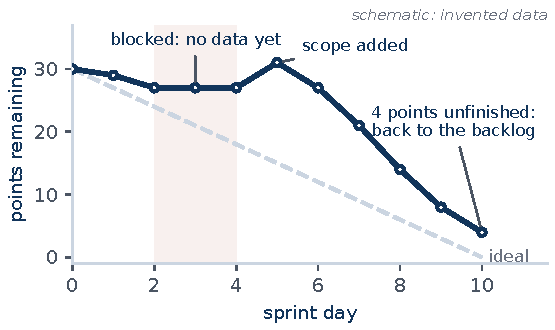
\includegraphics[height=3.4cm]{images/class25_burndown.pdf}\\[2pt]
\begin{tikzpicture}
\node[tileblue, anchor=north west, minimum width=6.4cm, text width=6.1cm, align=left, font=\scriptsize] at (0,0) {{\bfseries\color{courseblue}\faIcon{chart-line}\ How to read it.} A flat stretch means stuck or blocked work; a step up means scope was added; ending above zero means unfinished items go back to the backlog.};
\end{tikzpicture}
\column{0.49\textwidth}
\centering
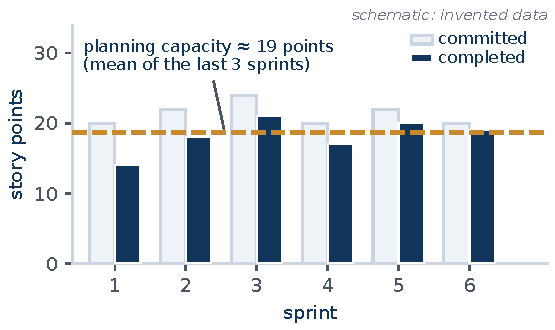
\includegraphics[height=3.4cm]{images/class25_velocity.pdf}\\[2pt]
\begin{tikzpicture}
\node[tilegold, anchor=north west, minimum width=6.4cm, text width=6.1cm, align=left, font=\scriptsize] at (0,0) {{\bfseries\goldink\faIcon{tachometer-alt}\ How to use it.} The recent average is the capacity for the next plan. Never compare teams, and never turn it into a target: Goodhart's law.};
\end{tikzpicture}
\end{columns}
\coursefooter
\end{cframe}

\begin{cframe}{Spikes: when the answer is unknown}{\cterm{Spike}{a time-boxed investigation that produces knowledge, not a feature.}}
\centering
\begin{tikzpicture}
\foreach \x/\ico/\col/\lab/\txt in {0/question-circle/courseblue/QUESTION/{Can a rolling mean spot drift early?}, 4.7/hourglass-half/coursegold/TIME-BOX/{One day, then stop and report.}, 9.4/clipboard-check/coursegreen/OUTPUT/{A notebook and a go or no-go call.}} {
  \node[tile, fill=white, draw=\col, thick, anchor=north west, minimum width=4.0cm, minimum height=1.2cm] at (\x,0) {};
  \badge{\x+0.55}{-0.6}{\col}{\ico}
  \node[anchor=north west, font=\tiny\bfseries, text=\col!80!black] at (\x+1.1,-0.12) {\lab};
  \node[anchor=north west, text width=2.75cm, align=left, font=\scriptsize] at (\x+1.1,-0.32) {\txt};
}
\draw[arrowgray] (4.05,-0.6) -- (4.65,-0.6);
\draw[arrowgray] (8.75,-0.6) -- (9.35,-0.6);
\node[chip, fill=courseblue, minimum width=5.5cm, minimum height=0.42cm, font=\scriptsize\bfseries, anchor=north west] at (2.15,-1.65) {\faIcon{sticky-note}\ STORY};
\node[chip, fill=coursegold, minimum width=5.5cm, minimum height=0.42cm, font=\scriptsize\bfseries, anchor=north west] at (7.8,-1.65) {\faIcon{flask}\ SPIKE};
\foreach \y/\lab/\a/\b in {-2.15/PURPOSE/{Deliver value to a user.}/{Reduce uncertainty.}, -2.8/SIZE/{Estimated in story points.}/{Time-boxed, not pointed.}, -3.45/DONE WHEN/{The acceptance criteria pass.}/{The question is answered with evidence.}} {
  \node[anchor=west, font=\tiny\bfseries, text=coursegray] at (0,\y-0.3) {\lab};
  \gridcell{2.15}{\y}{courseblue}{5.5}{\a}
  \gridcell{7.8}{\y}{coursegold}{5.5}{\b}
}
\keyidea{-4.4}{Modeling experiments are spikes by nature: time-box them, and agree in advance what evidence ends them (experiment tracking, Class 19).}
\end{tikzpicture}
\coursefooter
\end{cframe}

% ================================================================== PART 4
\sectiondivider{4}{Frameworks and failure modes}{project-diagram}{stories, boards, estimates, and charts make the work visible and measurable.}{$\bullet$\ Scrum, Kanban, and XP compared\\[3pt]$\bullet$\ Roles in an agile ML team\\[3pt]$\bullet$\ Feedback loops, from minutes to months\\[3pt]$\bullet$\ Anti-patterns in data and ML teams}

\begin{cframe}{Scrum, Kanban, XP: three centers of gravity}{\cterm{Kanban}{a method that manages continuous flow through visible work and WIP limits.}\cterm{DevOps}{shared responsibility of development and operations from build to run.}\cterm{MLOps}{DevOps extended with data, models, drift, and governance.}}
\centering
\begin{tikzpicture}
\foreach \x/\col/\ico/\name/\sub in {2.1/courseblue/sync-alt/Scrum/structured rhythm, 5.9/coursegreen/columns/Kanban/flow of work, 9.7/coursegold/code/Extreme Programming/engineering discipline} {
  \node[rounded corners=4pt, fill=\col, text=white, anchor=north west, minimum width=3.7cm, minimum height=0.9cm, align=center, font=\footnotesize\bfseries] at (\x,0) {\faIcon{\ico}\ \name\\[-1pt]{\scriptsize\mdseries\sub}};
}
\foreach \y/\lab in {-1.0/CADENCE, -1.8/ROLES, -2.6/KEY TOOLS, -3.4/FITS WHEN} {
  \node[anchor=west, font=\tiny\bfseries, text=coursegray] at (0,\y-0.36) {\lab};
}
\gridcell{2.1}{-1.0}{courseblue}{3.7}{Fixed-length sprints.}
\gridcell{5.9}{-1.0}{coursegreen}{3.7}{Continuous flow, no sprints.}
\gridcell{9.7}{-1.0}{coursegold}{3.7}{Weekly and quarterly planning cycles.}
\gridcell{2.1}{-1.8}{courseblue}{3.7}{Product Owner, Scrum Master, Developers.}
\gridcell{5.9}{-1.8}{coursegreen}{3.7}{No roles prescribed.}
\gridcell{9.7}{-1.8}{coursegold}{3.7}{The whole team, including the customer.}
\gridcell{2.1}{-2.6}{courseblue}{3.7}{Backlog, sprint, planning, review, retrospective.}
\gridcell{5.9}{-2.6}{coursegreen}{3.7}{Board, WIP limits, flow metrics.}
\gridcell{9.7}{-2.6}{coursegold}{3.7}{Pairing, TDD, continuous integration, refactoring.}
\gridcell{2.1}{-3.4}{courseblue}{3.7}{Cadence, as in student projects.}
\gridcell{5.9}{-3.4}{coursegreen}{3.7}{Continuous or varied work, as in operations.}
\gridcell{9.7}{-3.4}{coursegold}{3.7}{Code quality and fast technical feedback.}
\node[tilegold, anchor=north west, minimum width=13.4cm, minimum height=0.8cm, text width=12.6cm, align=left, font=\footnotesize] at (0,-4.4) {{\bfseries\goldink\faIcon{blender}\ Real teams mix them:} Scrum events, a Kanban board, XP practices. MLOps extends DevOps with data, models, drift, and governance.};
\end{tikzpicture}
\coursefooter
\end{cframe}

\begin{cframe}{Roles in an agile ML team}{\cterm{Product Owner}{the person accountable for the order of the backlog and the value of the product.}\cterm{Scrum Master}{the person who coaches the team in the process and removes impediments.}\cterm{Cross-functional team}{a team that holds all the skills needed to deliver an increment.}}
\centering
\begin{tikzpicture}
\foreach \y/\col/\ico/\name/\txt in {0/coursegold/user-tie/Product Owner/{Owns the order of the backlog and the value of the product; decides what comes next.}, -1.35/courseblue/user-shield/Scrum Master/{Coaches the team in the process and removes impediments; does not manage the work.}, -2.7/coursegreen/laptop-code/Developers/{Everyone who builds the increment: analysis, code, tests, data, and documentation.}} {
  \node[tileblue, draw=\col!80, anchor=north west, minimum width=8.0cm, minimum height=1.25cm] at (0,\y) {};
  \badge{0.65}{\y-0.625}{\col}{\ico}
  \node[anchor=west, text width=6.4cm, align=left, font=\small\bfseries, text=courseblue] at (1.25,\y-0.21) {\name};
  \node[anchor=north west, text width=6.4cm, align=left, font=\scriptsize, inner sep=0pt] at (1.25,\y-0.45) {\txt};
}
\node[anchor=west, font=\tiny\bfseries, text=coursegray] at (8.4,0.15) {THE SAME ROLES IN AN ML PRODUCT TEAM};
\foreach \y/\ico/\col/\name/\txt in {-0.45/flask/courseblue/Data scientist/{explores and models}, -1.1/cogs/coursegreen/ML engineer/{ships models}, -1.75/database/coursegold/Data engineer/{builds data pipelines}, -2.4/industry/coursered/Domain expert/{knows plant and data}} {
  \node[tile, fill=white, draw=\col!60, thick, anchor=west, minimum width=5.0cm, minimum height=0.52cm] at (8.4,\y) {};
  \node[circle, fill=\col, text=white, minimum size=0.4cm, inner sep=0, font=\scriptsize] at (8.7,\y) {\faIcon{\ico}};
  \node[anchor=west, font=\scriptsize\bfseries, text=courseblue] at (9.05,\y) {\name};
  \node[anchor=west, font=\tiny, text=coursegray] at (11.1,\y) {\txt};
}
\node[tilegold, anchor=north west, minimum width=5.0cm, minimum height=0.95cm, text width=4.7cm, align=left, font=\scriptsize] at (8.4,-2.85) {{\bfseries\goldink\faIcon{industry}\ Stakeholders} (operators, quality engineers) sit outside the team; the Product Owner speaks for them.};
\keyidea{-4.3}{Cross-functional means the skills to deliver an increment are inside the team: data, modeling, software, and operations. Roles name accountability, not job titles.}
\end{tikzpicture}
\coursefooter
\end{cframe}

\begin{cframe}{Feedback loops, from minutes to months}{\cterm{Feedback loop}{a cycle in which the results of work are observed and used to adjust the next step.}\cterm{Impact analysis}{tracing which requirements, tests, code, and documents a change touches.}}
\centering
\begin{tikzpicture}
\node[anchor=west, font=\tiny\bfseries, text=coursegray] at (0,0.15) {FEEDBACK LOOP};
\node[anchor=west, font=\tiny\bfseries, text=coursegray] at (3.5,0.15) {TIME UNTIL YOU KNOW (NOT TO SCALE)};
\node[anchor=west, font=\tiny\bfseries, text=coursegold!65!black] at (9.3,0.15) {WHAT IT CATCHES};
\fill[coursegold!12] (9.15,-3.45) rectangle (13.7,0.3);
\foreach \y/\ico/\col/\name/\len/\time/\txt in {-0.45/vial/coursegreen/Tests and CI/2.2/seconds to minutes/{a regression}, -1.05/user-friends/coursegreen/Pair and review/2.6/minutes to hours/{a logic or design error}, -1.65/sun/courseblue/Stand-up/3.0/one day/{a blocker}, -2.25/desktop/courseblue/Sprint review/4.0/one to four weeks/{the wrong thing built}, -2.85/history/courseblue/Retrospective/4.0/one to four weeks/{a wasteful way of working}, -3.45/chart-line/coursegold/Monitoring/5.5/months/{a world that has changed (drift)}} {
  \node[circle, fill=\col, text=white, minimum size=0.42cm, inner sep=0, font=\scriptsize] at (0.25,\y) {\faIcon{\ico}};
  \node[anchor=west, text width=2.7cm, align=left, font=\scriptsize\bfseries, text=courseblue] at (0.6,\y) {\name};
  \fill[\col, rounded corners=2pt] (3.5,\y-0.17) rectangle ({3.5+\len},\y+0.17);
  \node[anchor=west, font=\tiny\bfseries, text=white] at (3.58,\y) {\time};
  \node[anchor=west, text width=4.3cm, align=left, font=\scriptsize] at (9.3,\y) {\txt};
}
\keyidea{-3.95}{Shorter loops catch cheaper mistakes; only the longer ones catch the wrong requirement or a changed world. Change enters through the backlog, with its impact on requirements, tests, code, and documents made visible (Classes 22 and 26).}
\end{tikzpicture}
\coursefooter
\end{cframe}

\begin{cframe}{Agile anti-patterns in data and ML teams}{\cterm{Anti-pattern}{a common practice that looks helpful but backfires.}\cterm{Technical debt}{the future cost of shortcuts taken now.}}
\centering
\begin{tikzpicture}
\fill[coursegreen!8] (8.75,-3.75) rectangle (13.7,0.55);
\node[anchor=west, font=\tiny\bfseries, text=coursegray] at (0,0.3) {ANTI-PATTERN};
\node[anchor=west, font=\tiny\bfseries, text=coursegray] at (3.6,0.3) {WHAT HAPPENS};
\node[anchor=west, font=\tiny\bfseries, text=coursegreen] at (8.9,0.3) {A BETTER HABIT};
\aprow{-0.4}{flask}{Research as features}{Uncertain work is planned as routine implementation.}{Run a time-boxed spike that ends in evidence.}
\aprow{-1.15}{cloud}{Vague sprint items}{``Improve the model'' cannot be finished or tested.}{Write small, testable slices with criteria.}
\aprow{-1.9}{database}{Late data surprises}{Data dependencies surface only at integration.}{Put data access and quality in the Definition of Ready.}
\aprow{-2.65}{smile}{Happy-path demos}{Only what works is shown; the risk stays hidden.}{Demo evidence: replayed failures, edge cases, alert logs.}
\aprow{-3.4}{redo}{Retros without change}{Problems are named every sprint and nothing changes.}{One experiment, one owner, one date.}
\keyidea{-4.15}{Anti-patterns are shortcuts that feel like speed. In ML systems they pile up as technical debt: untested pipelines, undocumented data, models nobody can reproduce (Sculley et al., 2015).}
\end{tikzpicture}
\coursefooter
\end{cframe}

\begin{cframe}{What good agile behavior looks like in this course}{\cterm{Increment}{a usable piece of the system delivered at the end of a cycle (Class 23).}}
\centering
\begin{tikzpicture}
\goalcard{0}{0}{tileblue}{layer-group}{Demonstrate thin slices}{Ingest plus one rule plus one alert, not isolated fragments of three layers.}
\goalcard{6.8}{0}{tileblue}{columns}{Keep the board honest}{Requirements, deployment, docs, and validation all have cards.}
\goalcard{0}{-1.9}{tileblue}{search}{Make uncertainty visible}{Spikes, assumptions, and risks are listed as items, not hidden in heads.}
\goalcard{6.8}{-1.9}{tileblue}{sync-alt}{Feedback moves priorities}{Feedback re-orders the backlog; no first plan is ever complete.}
\keyidea{-3.95}{A requirement is not ``done'' merely because the Streamlit page renders. It needs reviewed code, acceptance evidence, and operational documentation: the Definition of Done from Class 23.}
\end{tikzpicture}
\coursefooter
\end{cframe}

% ------------------------------------------------------------------ closing
\section{Wrap-up}\gdef\currentsectionname{Wrap-up}
\begin{frame}{From this class to the next}
\centering
\begin{tikzpicture}
\foreach \i/\lab/\bg/\fg in {1/SE and ML/courseblue!22/courseblue, 2/Requirements/courseblue!22/courseblue, 3/Process/courseblue/white, 4/Design/courseice/coursegray, 5/Quality/courseice/coursegray, 6/Evolution/courseice/coursegray} {
  \node[rounded corners=3pt, minimum width=2.18cm, minimum height=0.6cm, font=\scriptsize\bfseries, fill=\bg, text=\fg] at ({1.1+(\i-1)*2.28},0) {\i\ \lab};
}
\node[font=\tiny\bfseries, text=courseblue] at (5.66,-0.52) {CLASS 23 AND THIS CLASS};
\foreach \x/\sty/\ico/\ttl/\txt in {0/tileblue/lightbulb/What stays with us/{$\bullet$\ Learn fast; keep the evidence.\\[3pt]$\bullet$\ Tools must reflect the data.\\[3pt]$\bullet$\ Thin slices beat notebooks.}, 4.55/tileblue/project-diagram/Use it in your project/{$\bullet$\ Organize milestones, backlog items, and reviews around deployable progress.\\[3pt]$\bullet$\ Pick the rituals and practices your team will really run.}, 9.1/tilegold/arrow-right/Next: Class 26/{\textbf{Pasteurization Monitoring Challenge.}\\[3pt]Your team specifies, builds, validates, and evolves a monitoring application against a live stream, using this toolkit.}} {
  \node[\sty, anchor=north west, minimum width=4.3cm, minimum height=3.8cm] at (\x,-0.95) {};
  \badge{\x+0.65}{-1.6}{courseblue}{\ico}
  \node[anchor=west, text width=3.0cm, align=left, font=\small\bfseries, text=courseblue] at (\x+1.2,-1.6) {\ttl};
  \node[anchor=north west, text width=3.9cm, align=left, font=\scriptsize] at (\x+0.2,-2.25) {\txt};
}
\node[tilegold, fill=white, anchor=north west, minimum width=13.4cm, minimum height=0.95cm, text width=12.6cm, align=left, font=\footnotesize] at (0,-5.0) {{\bfseries\goldink\faIcon{route}\ Course thread.} Agile coordination lets the team move continuously; sound engineering practices make that movement dependable.};
\end{tikzpicture}
\coursefooter
\end{frame}

% ------------------------------------------------------------------ references
\begin{frame}{References}
\centering
\begin{tikzpicture}
\refrow{0}{1.2}{book}{Books and guides}{Schwaber, K. and Sutherland, J. \href{https://www.scrumguides.org/}{The Scrum Guide}. \ \href{https://kanban.university/kanban-resources/getting-started/what-is-kanban/}{What is Kanban}.\\Beck, K. (2004). \emph{Extreme Programming Explained}, 2nd ed. Addison-Wesley.\\Stellman, A. and Greene, J. (2014). \href{https://www.oreilly.com/library/view/learning-agile/9780596527679/}{\emph{Learning Agile}}. O'Reilly.}
\refrow{-1.2}{1.1}{sticky-note}{Stories and planning}{Cohn, M. (2004). \emph{User Stories Applied}. Addison-Wesley.\\Wake, B. (2003). INVEST in Good Stories, and SMART Tasks.\\Fowler, M. \href{https://martinfowler.com/bliki/UserStory.html}{UserStory}.}
\refrow{-2.3}{2.2}{code}{Practices and delivery}{Beck, K. (2002). \emph{Test-Driven Development: By Example}. Addison-Wesley.\\Williams, L., Kessler, R., Cunningham, W., and Jeffries, R. (2000). Strengthening the Case for Pair Programming. \emph{IEEE Software}.\\Hannay, J. E. et al. (2009). The effectiveness of pair programming: a meta-analysis. \emph{Information and Software Technology}.\\Forsgren, N., Humble, J., and Kim, G. \href{https://itrevolution.com/product/accelerate/}{\emph{Accelerate}}.}
\refrow{-4.5}{1.3}{robot}{Data and ML}{Sculley, D. et al. (2015). \href{https://proceedings.neurips.cc/paper/2015/file/86df7dcfd896fcaf2674f757a2463eba-Paper.pdf}{Hidden Technical Debt in Machine Learning Systems}. NeurIPS.\\Breck, E. et al. (2017). The ML Test Score: A Rubric for ML Production Readiness and Technical Debt Reduction. \emph{IEEE Big Data}.}
\end{tikzpicture}
\coursefooter
\end{frame}

\end{document}
